\chapter{Requirements Engineering}
Quando si parla di \textbf{requirements engineering} (RE) di fatto ci si concentra
sulla comprensione di come una soluzione software si deve comportare per risolvere
un certo problema. In questo senso bisogna prima comprendere quale sia il problema
da risolvere e in quale contesto tale problema si verifica, per poter arrivare
ad una soluzione corretta ed efficacie a problemi reali. Non si parla quindi
della progettazione in se, ma del “cosa” deve fare il software.

Vediamo ora l'analogia classica per spiegare il requirements engineering,
rappresentata dal problema mondo e la soluzione macchina. Si hanno:
\begin{itemize}
      \item Il \textbf{mondo}, con un problema derivante dal mondo reale, esso
            stesso produce il problema che bisognerà risolvere con un calcolatore.
      \item La \textbf{macchina}: bisogna svilupparla per risolvere il problema.
      \item \textbf{Requirements engineering} che si occupa di definire gli effetti
            della macchina sul problema del mondo e definire assunzioni e proprietà
            principali del mondo stesso.
\end{itemize}
Macchina e mondo possono condividere alcuni componenti, con la macchina che
modifica il mondo. Nel requirements engineering studiamo quindi il mondo, senza
definire come funziona internamente la macchina.

Quando si parla di requirements engineering è bene distinguere due elementi:
\begin{itemize}
      \item Ogni volta che prendiamo in considerazione un problema esiste sempre
            un \textbf{system-as-is}, ovvero un sistema preesistente che già
            risolve il problema. Si ha quindi sempre un sistema da cui partire.
      \item \textbf{System-to-be}: ovvero il sistema che si andrà a realizzare.
            In altre parole è il sistema quando la macchina/software ci opera sopra.
\end{itemize}
Studiare il system-as-is è essenziale per poter lavorare al system-to-be.
\begin{definizione}[\textbf{Requirements engineering}]
      Il \textbf{requirements engineering} è, formalmente, un insieme di attività:
      \begin{itemize}
            \item Per esplorare, valutare, documentare, consolidare, rivisitare
                  e adattare gli obiettivi, le capacità, le qualità, i vincoli e
                  le ipotesi su un system-to-be.
            \item Basate sul problema sorto dal system-as-is e sulle nuove
                  opportunità tecnologiche.
      \end{itemize}
      L'output di queste attività è un documento di specifica dei requisiti con
      tutto ciò che soddisfa il sistema. Se l'output non è un singolo documento
      si ha una collezione di singoli requisiti, che nel metodo agile sono
      storie/cards e in altri metodi un repository centrale con un database
      condiviso contenete i vari requisiti.

      In ogni caso si ha un insieme di requisiti su come si deve comportare il
      sistema che si andrà a realizzare.
\end{definizione}
In un modello di sviluppo a cascata requirements engineering è una delle
primissime attività, subito dopo quelle di definizione del sistema e di business
plan.

Per gli aspetti tecnici è probabilmente la prima attività svolta, occupandosi di
ottenere il giusto sistema da sviluppare.

Un errore commesso in questa fase può portare ad un ottimo software che risolve
i problemi sbagliati oppure a un software che non risolve tutti i problemi che
dovrebbe risolvere.
\begin{center}
      Sbagliare il requirements engineering è una causa di fallimento del progetto.
\end{center}
Lavorare sui requirements non è semplice per diversi motivi:
\begin{itemize}
      \item Si deve ragionare su tante versioni del sistema come il system as-is,
            il system to-be e il system to-be-next, volendo essere lungimiranti
            per il comportamento del sistema, sapendo e prevedendo evoluzioni future.
      \item Si lavora in ambienti ibridi in un contesto che va compreso a fondo.
      \item Si hanno diversi aspetti funzionali, qualitativi e di sviluppo.
      \item Si hanno diversi livelli di astrazione, con obiettivi strategici a
            lungo termine di inserimento sul mercato e dettagli operazionali.
      \item Si hanno tanti stakeholders, quindi con diverse parti interessati di
            cui risolvere problemi e interessi con potenziali conflitti tra i
            vari stakeholders.
      \item Si hanno tante attività tecniche legate l'una con l'altra:
            \begin{itemize}
                  \item Conflict management
                  \item Risk management
                  \item Evaluation of alternatives
                  \item Prioritization
                  \item Quality assurance
                  \item Change anticipation
            \end{itemize}
\end{itemize}
\section{Tipi di requisiti}
Bisogna anche ragionare sui tipi di requisiti su cui si deve lavorare. Una prima
differenza si ha nel modo in cui sono scritti i requisiti. Si hanno quindi:
\begin{itemize}
      \item \textbf{Descriptive statements}: rappresentano i requisiti non
            negoziabili, ovvero dei comportamenti derivanti dalle leggi del mondo
            su cui si lavora. Si ha quindi zero margine di modifica.
      \item \textbf{Prescriptive statements}: indicano requisiti negoziabili.
\end{itemize}
Entrambi sono importanti e vanno considerati. Spesso si possono avere dei
requisiti che chi lavora nell'ambiente da per scontato, ma chi invece lavora sul
software non conosce.

I requisiti possono inoltre differire per gli elementi che prendono in considerazione.
In particolare, si possono avere:
\begin{itemize}
      \item \textbf{System requirements}: come si comporta l'ambiente, per capirne
            il funzionamento.
      \item \textbf{Software requirements}: come si comporta il software
            nell'ambiente, studiando i cosiddetti \textit{shared fenomena}.
\end{itemize}
ricordando che:
\begin{center}
      Sistema = Ambiente + Software
\end{center}
\begin{center}
      System requirements = Software requirements + Domain Properties + Assumption
\end{center}
I requisti comunque non riguardano mai il comportamento interno del software.

Si hanno 3 dimensioni:
\begin{enumerate}
      \item \textbf{Dimensione del why}: si identificano, analizzano e rifiniscono
            i requisiti del system-to-be con lo scopo di affrontare le carenze
            analizzate del system-as-is, in linea con gli obiettivi di business,
            sfruttando le opportunità tecnologiche. Si hanno le seguenti difficoltà:
            \begin{itemize}
                  \item Acquisire conoscenza del dominio.
                  \item Valutare opzioni alternative.
                  \item Abbinare problemi-opportunità e valutarli in termini di
                        implicazioni, e rischi associati.
                  \item Gestire obiettivi contrastanti.
            \end{itemize}
      \item \textbf{Dimensione del what}: si identificano, analizzano e rifiniscono
            le funzionalità del system-to-be per soddisfare gli obiettivi
            individuati in base a vincoli basati su ipotesi realistiche
            sull'ambiente. Si hanno le seguenti difficoltà:
            \begin{itemize}
                  \item Identificare il giusto set di funzionalità.
                  \item Specificarle precisamente per essere comprese da tutte
                        le parti.
                  \item Garantire la tracciabilità backward per gli obiettivi
                        del sistema.
            \end{itemize}
      \item \textbf{Dimensione del who}: si assegna responsabilità per gli
            obiettivi, i servizi, i vincoli tra i componenti del system-to-be in
            base alle loro capacità e agli obiettivi del sistema, oltre i confini
            dell'ambiente software. La difficoltà è valutare opzioni alternative
            per decidere il giusto grado di automazione.
\end{enumerate}
I requisti che riguardano l'ambiente possono essere di due forme:
\begin{itemize}
      \item \textbf{Domain properties}: proprietà riguardanti l'ambiente, queste
            sono immutabili.
      \item \textbf{Assumptions}: su come è fatto l'ambiente. Il software
            funzionerà solo negli ambienti che soddisfano quella certa assunzione.
            Se troppo restrittive possono portare al fallimento del progetto,
            che riguarderebbe pochissimi casi particolari.
\end{itemize}
\begin{definizione}[\textbf{Domain property}]
      Definiamo \textbf{domain property} come un descriptive statement sui problemi
      legati ai fenomeni del mondo, a prescindere da qualsiasi software-to-be.
      \begin{equation}
            \text{Domain property} \ \subseteq M \times C
      \end{equation}
      se leggi che non possono essere infrante.
\end{definizione}
Si ha che:
\begin{center}
      Software requirements = \textit{map}(System requirements, Software
      requirements, Domain property)
\end{center}
È utile quindi fare una distinzione per quanto concerne i requisiti del software.
Abbiamo due famiglie principali di requisiti:
\begin{itemize}
      \item \textbf{Requisiti funzionali}: che indicano le funzionalità che un
            sistema (system-to-be) deve implementare, cosa deve essere in grado
            di fare. Non sono prevedibili prima di studiare il sistema.
      \item \textbf{Requisiti non funzionali}: che indicano delle qualità o dei
            vincoli sulle funzionalità e quindi sui requisiti funzionali. Questa
            famiglia di aspetti non funzionali è più o meno standard.
\end{itemize}
Per l'identificazione dei requisiti non funzionali si può utilizzare una
\textit{tassonomia}, riportata in figura \ref{fig:tasso}, dove si trovano
organizzati aspetti non funzionali tali per cui, dopo aver individuato le
funzionalità posso ricercare eventuali requisiti non funzionali.
\begin{figure}[!ht]
      \centering
      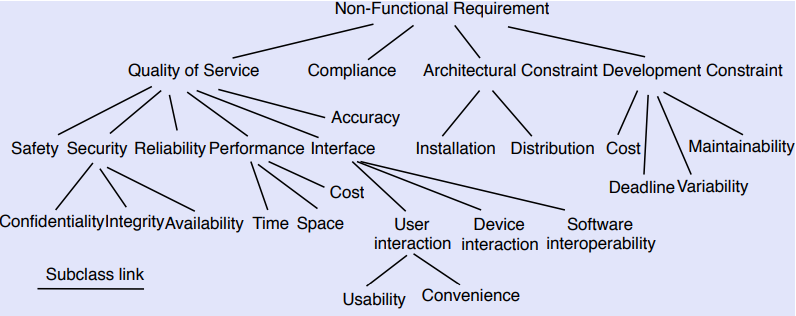
\includegraphics[width=0.5\textwidth]{img/requirements/tassonomia.png}
      \caption{Tassonomia dei requisiti non funzionali}
      \label{fig:tasso}
\end{figure}
Per alcuni tipi di progetti requisiti funzionali e non funzionali sono
difficilmente distinguibili, spesso c'è il rischio che siano mischiati.

Le interazioni tra l'ambiente e sistema si possono effettuare secondo lo schema
riportato in figura \ref{fig:int-sistema-ambiente}.
\begin{figure}[!ht]
      \centering
      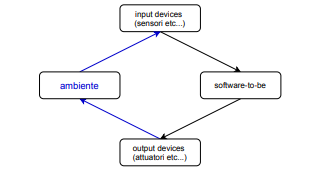
\includegraphics[width=0.5\textwidth]{img/requirements/interazione-sistema-ambiente.png}
      \caption{Schema delle interazioni tra sistema e ambiente}
      \label{fig:int-sistema-ambiente}
\end{figure}
Lo scambio di informazioni avviene mediante gli I/O device e 4 tipologie di variabili:
\begin{itemize}
      \item \textbf{Input data} ($I$): variabili tra input device e software-to-be.
      \item \textbf{Output results} ($O$): variabili tra software-to-be e output
            device.
      \item \textbf{Controlled variables} ($C$): variabili tra output device e
            ambiente.
      \item \textbf{Monitored variables} ($M$): variabili tra ambiente e input
            device.
\end{itemize}
I requisiti introdotti precedentemente sono in relazione con queste variabili.
In particolare abbiamo:
\begin{equation}
      \begin{array}{l}
            \text{System requirements} \subseteq M \times C                        \\
            \text{Software requirements} \subseteq I \times O                      \\
            \text{Assunzioni} \subseteq M \times C \cup M \times I \cup C \times O \\
            \text{Domain property}\subseteq M\times C
      \end{array}
\end{equation}
\section{Qualità dei requisiti}
Si hanno diversi aspetti di cui preoccuparsi nell'analisi dei requisiti. Tra i
principali abbiamo:
\begin{itemize}
      \item \textbf{Completezza}: è necessario descrivere tutti i requisiti
            rilevanti del progetto, identificando tutti i comportamenti del sistema
            e documentarli in modo adeguato. È una qualità virtualmente
            irraggiungibile in modo assoluto, non è infatti verificabile. Inoltre
            i requisiti variano al proseguire del progetto, interagendo anche
            con gli stakeholders, rendendo questo uno degli aspetti più difficili
            da studiare.
      \item \textbf{Consistenza}: i requisiti non devono presentare dei conflitti,
            dato l'elevato numero di requisiti è facile introdurre inconsistenze.
      \item \textbf{Non ambiguità}: tutto deve essere chiaro e non soggetto ad
            interpretazione.
      \item \textbf{Misurabilità}: ogni requisito non deve essere basato su
            interpretazioni vaghe ma bensì su misure concrete e specifiche.
      \item \textbf{Fattibilità}: non si devono avere requisiti basati su
            funzionalità irrealizzabili.
      \item \textbf{Comprensibilità}.
      \item \textbf{Buona struttura}.
      \item \textbf{Modificabilità}: possibilità di avere il risultato mantenibile
            del tempo.
      \item \textbf{Tracciabilità}: individuando tutti gli artefatti ottenibili
            come conseguenza e tracciandoli. Si tracciano anche le dipendenze
            tra requisiti.
\end{itemize}
Vediamo quindi gli errori che si fanno quando si va ad identificare i requisiti:
\begin{itemize}
      \item \textbf{Omissioni}: non si riesce ad identificare qualche requisito.
            Anche un riconoscimento tardivo è un problema in quanto comporta la
            modifica del documento, non sempre facile.
      \item \textbf{Contraddizioni}: si presentano conflitti tra i requisiti.
      \item \textbf{Inadeguatezza}: requisiti che non sono adeguati per un
            determinato problema.
      \item \textbf{Ambiguità}: requisiti interpretabili.
      \item \textbf{Non misurabilità}: non si riesce a fornire una misura di
            certi requisiti, specialmente non funzionali, che comportano
            difficoltà di gestione.
\end{itemize}
Si hanno anche altri tipi di errore:
\begin{itemize}
      \item Essere troppo specifici nella definizione dei requisiti includendo
            anche comportamenti interni al software che non dovrebbero essere
            descritti in questa fase.
      \item Descrivere requisiti non implementabili considerando vincoli
            temporali o di costo.
      \item Descrivere requisti complessi da leggere.
      \item Avere poca struttura nella stesura dei requisiti, a livello visivo.
      \item Se si produce un documento bisogna evitare di fare riferimento a
            requisiti che non sono stati ancora descritti, ovvero evitando il
            \textit{forward reference}.
      \item Evitare “rimorsi” di non aver definito nel momento giusto certi
            concetti che magari erano stati usati, senza definizione, precedentemente.
      \item Evitare la poco modificabilità del documento. È buona norma avere
            delle “costanti simboliche”, definite all'inizio, a cui fare
            riferimento nel documento, in modo che un'eventuale modifica si
            rifletta su tutto il documento.
      \item Evitare l'opacità/logica di fondo/rationale/motivazioni dei requisti,
            in modo che sia chiaro il perché esso è stato incluso, portando a
            mettere in discussione requisiti in realtà sensati a cui si arriverebbe
            comunque dopo ulteriore analisi, dopo aver perso ulteriore tempo.
\end{itemize}
\section{Il processo requirements engineering}
Il processo di requirements engineering è composto da 4 fasi che seguono una
struttura a spirale, come riportato in figura \ref{fig:spirale}:
\begin{figure}[!ht]
      \centering
      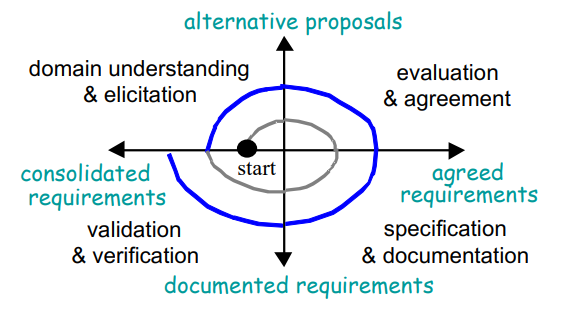
\includegraphics[width=0.6\textwidth]{img/requirements/spirale.png}
      \caption{Rappresentazione modello a spirale}
      \label{fig:spirale}
\end{figure}
\begin{enumerate}
      \item \textbf{Domain understanding} $\&$ \textbf{elicitation}: in questa
            fase si hanno due parti principali:
            \begin{itemize}
                  \item \textbf{Domain understanding}: in questa fase si ha lo
                        studio del system-as-is in ottica di studio del dominio
                        applicativo, studio del business organizzazione che vuole
                        il prodotto. Si studiano anche forze e debolezze del
                        system-as-is. Si studia il dominio applicativo per ottenere
                        il miglior system-to-be possibile. Inoltre, si
                        identificano gli stakeholders del progetto per poter
                        capire a fondo interessi e fini.

                        Come output di questa fase si hanno le sezioni iniziali
                        per la bozza di proposta preliminare e il glossario dei
                        termini.
                  \item \textbf{Requirements elicitation}: studio più approfondito
                        nel mondo attraverso un'ulteriore analisi dei problemi
                        legati al system-as-is. Inoltre, vengono identificati,
                        grazie all'aiuto degli stakeholders:
                        \begin{itemize}
                              \item Opportunità tecnologiche
                              \item Condizioni del mercato
                              \item Obiettivi di miglioramento
                              \item Vincoli, organizzativi e tecnici, del system-as-is
                              \item Alternative per raggiungere l'obiettivo e
                                    assegnare le responsabilità.
                              \item Scenari di ipotetica interazione software-ambiente
                              \item Requisiti del software
                              \item Assunzioni sull'ambiente
                        \end{itemize}
                        In in output si hanno ulteriori sezioni per la bozza di
                        proposta preliminare.
            \end{itemize}
      \item \textbf{Evaluation} $\&$ \textbf{agreement}: si effettuano decisioni
            basate sull'interazione con i vari stakeholders, per poter valutare
            e decidere, avendo cambiamenti dei rischi in base a:
            \begin{itemize}
                  \item Identificazione e risoluzione di conflitti di interesse.
                  \item Identificazione e risoluzione di rischi legati al sistema
                        proposto.
                  \item Comparazione e scelta tra le alternative proposte in
                        merito a obiettivi e rischi.
                  \item Prioritization dei requisti, al fine di risolvere
                        conflitti, definire vincoli di costi e tempi, supportare
                        lo sviluppo incrementale.
            \end{itemize}
            In in output a questa fase si hanno le sezioni finali per la bozza
            di proposta preliminare, dove si documentano gli obiettivi selezionati,
            i requisiti, le assunzioni e il rationale, la logica di fondo delle
            opzioni selezionate.
      \item \textbf{Specification} $\&$ \textbf{documentation}: in questa fase
            si raccoglie quanto detto nelle prime due fasi per produrre il
            documento, si hanno quindi:
            \begin{itemize}
                  \item Definizione precisa di tutte le funzionalità del sistema
                        scelto, tra cui:
                        \begin{itemize}
                              \item Obiettivi, concetti, proprietà rilevanti del
                                    dominio d'interesse, requisti del sistema,
                                    requisti del software, assunzioni sull'ambiente
                                    e responsabilità.
                              \item Motivazioni e logica di fondo delle opzioni
                                    scelte.
                              \item Probabili evoluzioni del sistema ed eventuali
                                    variazioni.
                        \end{itemize}
                  \item Organizzazione di quanto appena citato in una struttura
                        coerente.
                  \item Documentazione del tutto in un formato comprensibile a
                        tutte le parti, mettendo in allegato:
                        \begin{itemize}
                              \item Costi
                              \item Piano di lavoro
                              \item Tempi di consegna del risultato
                        \end{itemize}
            \end{itemize}
            In output a questa fase si ha il vero e proprio \textbf{Requirements
                  Document} (RD).
      \item \textbf{Validation} $\&$ \textbf{verification}: in questa fase si
            studia il requirements document, ovvero si studia la garanzia di
            qualità del requirements document, analizzando varie attività:
            \begin{itemize}
                  \item Validazione, ovvero vedendo se quanto contenuto nel
                        requirements document è adeguato con quanto si necessita.
                  \item Verifica, controllando se ci sono omissioni o
                        inconsistenze.
                  \item Correzione di eventuali errori e difetti.
            \end{itemize}
            In output a questa fase si ha un requirements document consolidato.
\end{enumerate}
Come è stato detto queste quattro fasi si ripetono in modo iterativo. Questo
viene fatto in quanto si possono avere evoluzioni nel processo nonché correzioni
di quanto già fatto che si propagano su tutto il documento. Le evoluzioni e le
correzioni possono sopraggiungere durante:
\begin{itemize}
      \item Il requirements engineering stesso.
      \item Lo sviluppo del software.
      \item Dopo il deploy del software stesso.
\end{itemize}
Dopo ogni ciclo si è molto più consci del sistema e si può passare al miglioramento
del requirements engineering con più efficacia.
\subsection{Domain understanding \& elicitation}
Iniziamo analizzando la fase di \textbf{elicitation}, la quale consiste in un
insieme di tecniche atte allo scoprire requisiti che un progetto deve soddisfare.
\subsubsection{Stakeholders}
La selezione degli stakeholders del progetto è la prima fase che viene svolta
per poter lavorare alla elicitation.
\begin{definizione}[\textbf{Stakeholder}]
      In generale uno \textbf{stakeholder} è un'organizzazione o una persona che
      nutre un interesse rispetto al progetto. Si hanno diversi aspetti per la
      selezione degli stessi:
      \begin{itemize}
            \item Posizione nell'organizzazione.
            \item Ruolo nel prendere decisioni sul system-to-be.
            \item Livello di esperienza del dominio applicativo.
            \item Esposizione al problema che il sistema deve risolvere.
            \item Influenza nell'accettazione del sistema.
            \item Obiettivi personali ed eventuali conflitti di interesse.
      \end{itemize}
\end{definizione}
Conoscendo gli stakeholders avremo modo di prendere in considerazioni gli
interessi di essi tramite diverse strategie. Idealmente si vuole realizzare
qualcosa che soddisfi gli interessi di tutti.

Questa è un'attività insidiosa in quanto non si può dire se l'insieme degli
stakeholders sia completo. Si hanno anche stakeholders che non sono
dell'organizzazione o che non interagiscono direttamente col sistema.

Un modo per identificare gli stakeholders è tramite una serie di semplici
domande, poste durante una piccola attività di brainstorming:
\begin{itemize}
      \item Chi è influenzato positivamente e negativamente dal progetto?
      \item Chi ha il potere di fargli avere successo (o farlo fallire)?
      \item Chi prende le decisioni in materia di denaro?
      \item Chi sono i fornitori?
      \item Chi sono gli utenti finali?
      \item Chi ha influenza, anche indiretta, sugli altri stakeholder?
      \item Chi potrebbe risolvere potenziali problemi con il progetto?
      \item Chi si occupa di assegnare o procurare risorse o strutture?
      \item Chi ha competenze specialistiche cruciali per il progetto?
\end{itemize}
Dimenticare uno stakeholders può portare ritardi o fallimenti del progetto,
dovendo rivedere magari requisti o dovendo rifare parti di sviluppo. Si hanno
varie difficoltà nell'acquisire informazioni dagli stakeholders, rendendo
complesso il dialogo:
\begin{itemize}
      \item Fonti di conoscenza sul sistema distribuite sui vari stakeholders e
            tali fonti spesso sono contrastanti.
      \item Accesso difficile alle fonti.
      \item Ostacoli alla buona comunicazione, avendo background diversi sul
            dominio.
      \item Conoscenza non comunicata esplicitamente e bisogni nascosti.
      \item Fattori socio-politici.
      \item Condizioni instabili e mutabili, cambiano gli stakeholders, si hanno
            dinamiche aziendale mutevoli e cambi di ruoli. Anche per questo si
            hanno i metodi agili.
\end{itemize}
Servono quindi buone capacità comunicative, sapendo usare la giusta terminologia
di dominio, arrivando dritti al punto e creando un rapporto di fiducia con gli
stakeholders. Si ha inoltre un piccola pratica, detta \textbf{knowledge reformulation},
ovvero quando si acquisiscono informazioni anche da fonti multiple è bene
riformulare tale informazione allo stakeholder, per verificare una corretta
comprensione.

È bene fare distinzione sulle tecniche di engagement con gli stakeholders,
considerando due variabili, catalogandole in low e high:
\begin{enumerate}
      \item \textbf{Potere decisionale}.
      \item \textbf{Interesse nel progetto}.
\end{enumerate}
Si ha quindi una classificazione degli stakeholders in base a queste due variabili:
\begin{table}[!ht]
      \centering
      \begin{tabular}{c|c|c}
            \textbf{Potere} & \textbf{Interesse} & \textbf{Strategia} \\\hline
            high            & high               & Fully engage       \\
            high            & low                & Keep satisfied     \\
            low             & high               & Keep satisfied     \\
            low             & low                & Minimum effort
      \end{tabular}
\end{table}
Dove nel dettaglio:
\begin{itemize}
      \item \textbf{Fully engage}: implica un coinvolgimento regolare degli
            stakeholders che in questo caso sono della categoria principale.
      \item \textbf{Keep satisfied}: si hanno due casi:
            \begin{itemize}
                  \item Se hanno alto potere decisionale si cerca di mantenerli
                        informati e soddisfatti ma senza troppi dettagli.
                  \item Se hanno alto interesse, essendo spesso gli end-user, si
                        cerca di consultarli spesso cercando di risolvere le
                        problematiche indicate, coinvolgendoli regolarmente per
                        ottenere dettagli e informazioni specifiche, essendo
                        spesso i più informati sui dettagli.
            \end{itemize}
      \item \textbf{Minimum effort}: mentendoli informati in modo generale e
            monitorandone eventuali cambi di ruolo, potere o interesse.
\end{itemize}
\subsubsection{Elicitation techniques}
Passiamo quindi alle tecniche di elicitation. Si hanno due famiglie principali:
\begin{itemize}
      \item \textbf{Artefact-driven}: uso di artefatti per poter scoprire requisiti.
            \begin{enumerate}
                  \item \textbf{Background study}: ovvero collezionare leggere
                        e sintetizzare documenti su:
                        \begin{itemize}
                              \item Le organizzazioni stesse.
                              \item Il dominio applicativo.
                              \item Il system-as-is, ovvero workflow documentati,
                                    procedure, regole di business, report di
                                    errori, richieste di cambiamenti $\dots$
                        \end{itemize}
                        Queste collezioni di dati ci permettono di informarci in
                        modo autonomo sul mondo in cui si andrà a lavorare, senza
                        coinvolgere lo stakeholders, in quanto costoso, dispendioso
                        e limitato in termini di tempo. Gli stakeholders vanno
                        interpellati non per informazioni reperibili autonomamente
                        ma per estrarre conoscenza non pubblica e non documentata.
                        Ci si presenta allo stakeholder già con una base di
                        conoscenza e conoscendo già la terminologia corretta del
                        dominio.

                        Si ha quindi l'attività di data collection dove si
                        estraggono informazioni utili per studiare il target. Si
                        possono fare attività di survey. Si collezionano dati anche
                        già documentati.

                        L'attività di background study ha ovviamente dei limiti
                        di scalabilità, non potendo leggere troppe cose, sia per
                        tempo, sia per costo. Si ha quindi la meta-knowledge per
                        selezionare le parti dei documenti più rilevanti.
                        Queste attività sono essenziali all'avvio di un progetto.

                        Quindi il \textbf{pro} principale è che si ottengono
                        informazioni di base per interagire con gli stakeholder,
                        perché permette di chiedere direttamente informazioni non
                        banali. Il \textbf{contro} principale è che bisogna
                        analizzare tanti documenti e questa è un operazione
                        costosa, le informazioni di interesse sono solo una
                        piccolissima parte, quindi bisogna avere un minimo di
                        intuito per selezionare velocemente le informazioni rilevanti.
                  \item \textbf{Questionari}: si sottomette una lista di domande
                        chiuse agli stakeholder, ogni domanda sarà misurabile
                        quantitativamente (percentuali) e qualitativamente. I
                        questionari sono perfetti per ottenere velocemente,
                        economicamente e a distanza informazioni da molte persone,
                        sono utilizzati per prepararsi bene alle interview. I
                        problemi sul loro utilizzo sono:
                        \begin{itemize}
                              \item Bias nelle domande: si danno per scontate
                                    delle informazioni.
                              \item Informazioni inaffidabili: spesso ci possono
                                    essere informazioni mal interpretate e risposte
                                    inconsistenti.
                        \end{itemize}
                        Le linee guida sono:
                        \begin{itemize}
                              \item Identificare un gruppo statisticamente
                                    significativo di persone.
                              \item Controllare la copertura delle domande e delle
                                    risposte.
                              \item Controllare che le domande e le risposte siano
                                    non ambigue e senza bias.
                              \item Aggiungere domande ridondanti per identificare
                                    risposte inconsistenti.
                              \item Controllare il questionario da un'altra persona.
                        \end{itemize}
                  \item \textbf{Storyboards}: narrazioni, tramite esempi, di uso
                        del sistema, sia del system-as-is che del system-to-be.
                        Sono quindi storie fatte tramite sequenze di snapshots.
                        Tali storie si creano in due modi:
                        \begin{itemize}
                              \item \textbf{Attivo}, dove lo stakeholder contribuisce
                                    alla costruzione della narrazione.
                              \item \textbf{Passivo}, dove si narra la storia
                                    costruita allo stakeholder.
                        \end{itemize}
                        Ovviamente vengono fatte solo per i workflow chiari.
                  \item \textbf{Scenari}: descrivono, attraverso una sequenza di
                        interazioni rappresentate con testi o diagrammi, l'utilizzo
                        del sistema, sia as-is, sia to-be. L'uso di esempi rende
                        semplice la comunicazione e l'interazione con gli altri.
                        Si hanno 4 tipi di scenario:
                        \begin{itemize}
                              \item \textbf{Positivo}, ovvero come il sistema si
                                    dovrebbe comportare, si dividono in:
                                    \begin{itemize}
                                          \item \textbf{Normale}: ovvero tutto
                                                procede come dovrebbe.
                                          \item \textbf{Anormale}: ovvero cosa
                                                succede in casi eccezionali.
                                    \end{itemize}
                              \item \textbf{Negativo}: ovvero cosa il sistema
                                    non dovrebbe fare.
                        \end{itemize}
                        I \textbf{pro} sono che si hanno esempi e controesempi
                        concreti, usabili per i test case e piacciono agli
                        stakeholders.

                        I \textbf{contro} sono che non sono completi, si ha
                        un'esplosione combinatoria, potenzialmente inutilmente
                        specifici, spesso la sequenza descritta non deve essere
                        per forza mantenuta nel futuro sistema, molti dettagli
                        irrilevanti e incompatibili dettagli da diversi
                        stakeholders.
                  \item \textbf{Prototipi} e \textbf{mock-up}: sono realizzati
                        quando l'obiettivo è quello di controllare l'adeguatezza
                        di un requisito, che viene mostrato in modo visuale nella
                        sua ipotetica formula finale. Si hanno quindi piccoli
                        esempi del software in azione, chiarendo e verificando
                        che sia quello di cui l'utente ha bisogno. Ovviamente un
                        mock-up non ha la logica applicativa, ma ha risposte costruite
                        a priori. A seconda del tipo di mock-up il focus è su:
                        \begin{itemize}
                              \item \textbf{Funzionale}: funzionalità, se sono
                                    state comprese correttamente e in modo
                                    esaustivo.
                              \item \textbf{UI}: UI e UX, avendo focus più
                                    orientati all'usabilità.
                        \end{itemize}
                        Si parla di mock-up se dopo l'uso viene buttato e di
                        prototipo se, in caso di approvazione, viene usato come
                        base del software o comunque riutilizzato in qualche modo,
                        fornendo eventualmente una base evolutiva del software
                        finale.

                        I \textbf{pro} sono che si ha un idea concreta di cosa
                        il software farà e come sarà, chiarisce i requisiti e
                        mostra quelli nascosti, migliora l'accettabilità.

                        I \textbf{contro} sono che possono creare aspettative
                        troppo alte come tempi di risposta istantanei, quando in
                        realtà non si ha implementato nulla, il codice è molto
                        sporco difficile da riutilizzare per il software finale
                        e, infine, sono costosi.
                  \item \textbf{knowledge reuse}: per velocizzare l'elicitation,
                        si riusano conoscenze pregresse da sistemi simili a quello
                        sotto studio. Si hanno 3 fasi:
                        \begin{enumerate}
                              \item Trarre conoscenze e informazioni rilevanti
                                    da altri sistemi.
                              \item Trasporle nel sistema in studio.
                              \item Convalidare il risultato, adattarlo se
                                    necessario e integrarlo con la conoscenza del
                                    sistema già acquisita.
                        \end{enumerate}
                        Tali conoscenze possono essere dipendenti o indipendenti
                        dal dominio. Si hanno i seguenti \textbf{pro}:
                        \begin{itemize}
                              \item Analisti esperti riutilizzano naturalmente
                                    dall'esperienza passata.
                              \item Riduzione degli sforzi di elicitation.
                              \item Ereditarietà della struttura e qualità delle
                                    specifiche del dominio astratto.
                              \item Efficace per completare i requisiti con aspetti
                                    trascurati.
                        \end{itemize}
                        e i seguenti \textbf{contro}:
                        \begin{itemize}
                              \item Efficace solo se il dominio astratto è
                                    sufficientemente simile e accurato.
                              \item Definire domini astratti per una riusabilità
                                    significativa è difficile.
                              \item Si hanno forti sforzi di convalida e integrazione.
                              \item Le corrispondenze vicine possono richiedere
                                    adattamenti complicati.
                        \end{itemize}
                  \item \textbf{Card sort}: che consiste nel chiedere agli
                        stakeholder di suddividere un set di carte dove:
                        \begin{itemize}
                              \item Ogni carta cattura un concetto in modo testuale
                                    o grafico.
                              \item Carte raggruppate in sottoinsiemi in base ai
                                    criteri degli stakeholder.
                        \end{itemize}
                        L'obiettivo è acquisire ulteriori informazioni sui
                        concetti già evocati. Per ogni sottoinsieme, chiedere la
                        proprietà condivisa implicita utilizzata per il
                        raggruppamento per poi ripetere con le stesse carte per
                        nuovi raggruppamenti / proprietà.
            \end{enumerate}
      \item \textbf{Stakeholders-driven}: fanno invece uso degli stakeholders.
            \begin{enumerate}
                  \item \textbf{Intervista} che consiste in:
                        \begin{itemize}
                              \item Selezione mirata dello stakeholder, in base
                                    alle informazioni necessarie.
                              \item Fare l'intervista registrando le risposte.
                              \item Scrivere il transcript dell'intervista e
                                    produrre subito il report.
                              \item Sottomettere all'intervistato il report per
                                    validazione.
                        \end{itemize}
                        Si può avere un'intervista anche con più stakeholder.
                        L'intervista è una tecnica costosa e le interviste possono
                        essere poche, bisogna quindi procedere in modo attento.
                        Si hanno due tipi di interviste:
                        \begin{itemize}
                              \item \textbf{Strutturate}: si parte con un insieme
                                    di domande già scelto per un certo obiettivo.
                                    Si da poco spazio ad una discussione aperta.
                              \item \textbf{Non strutturate}: si da spazio alla
                                    discussione aperta e libera sul system-as-is,
                                    sulle problematiche e sulle soluzioni.
                        \end{itemize}
                        Spesso si hanno interviste miste, nella prima parte
                        strutturate e poi con domande e argomenti liberi. Gli
                        argomenti vanno calibrati così come il numero di domande,
                        per evitare perdite di tempo e di attenzione da parte
                        dello stakeholder. Vediamo quindi qualche linea guida per
                        la preparazione delle interviste.
                        \begin{itemize}
                              \item Bisogna arrivare preparati, tramite il
                                    background study.
                              \item Per costruire un rapporto con lo stakeholder
                                    le domande devono essere su misura dello stesso,
                                    in base al suo lavoro e ruolo.
                              \item Mettere in centro dell'intervista le necessità
                                    e problematiche dell'intervistato, chiarendo
                                    di essere interessati al suo punto di vista.
                              \item Evitare che la discussioni dilagazioni su argomenti
                                    inutili.
                              \item Fare in modo che l'intervistato si senta a
                                    suo agio, magari iniziando con qualche
                                    chiacchiera informale e domande semplici per
                                    poi spostarsi su domande difficili.
                              \item Dimostrarsi affidabile.
                              \item Chiedere sempre “perché” cercando il rationale
                                    di ciò che si chiede.
                              \item Evitare domande bias che influenzino la risposta.
                              \item Evitare domande ovvie che facciano pensare
                                    all'intervistato che stia perdendo tempo.
                              \item Evitare domande a cui sicuramente l'intervistato
                                    non sa rispondere.
                        \end{itemize}
                        Nel \textit{transcript} bisogna includere reazioni personali.
                  \item \textbf{Studi osservazionali ed etnografici}: studi che
                        si basano sull'osservazione degli stakeholders stessi
                        all'azione, nell'ottica del system-as-is, osservando come
                        svolgono vari task per cogliere problemi e funzionalità.
                        Si hanno due modalità di osservazione:
                        \begin{itemize}
                              \item \textbf{Osservazione passiva}: non si produce
                                    interferenza sulle azioni dello stakeholder,
                                    guardando da fuori, registrando record e
                                    producendo un transcript. Si hanno due particolari
                                    osservazioni passive:
                                    \begin{enumerate}
                                          \item \textbf{Protocol analysis}: si
                                                studia qualcuno che svolge un
                                                certo protocollo, un certo task.
                                          \item \textbf{Ethnographic studies}:
                                                studio che si svolge in un lungo
                                                periodo di tempo, dove si prova
                                                a scoprire le proprietà emergenti
                                                del gruppo sociale coinvolto.
                                    \end{enumerate}
                              \item \textbf{Osservazione attiva}: dove si svolge
                                    in prima persona i task, diventando eventualmente
                                    team member, capendo attivamente come deve
                                    essere svolto un task.
                        \end{itemize}
                        I \textbf{pro} sono che si può scoprire la \textbf{tacit
                              knowledge} emergente e i \textbf{problemi nascosti},
                        in aggiunta si ha una \textbf{contestualizzazione} delle
                        informazioni acquisite.

                        I \textbf{contro} sono che è \textbf{lento e costoso},
                        deve essere fatto su un lungo periodo e in differenti
                        tempi, con diversi carichi di lavoro. Potrebbe essere
                        \textbf{inaccurato} perché le persone potrebbero lavorare
                        diversamente perché osservate e si ha un focus sul
                        system-as-is.
                  \item \textbf{Group sessions}: ovvero una famiglia di tecniche
                        utili per la risoluzione di conflitti. L'elicitation prende
                        la forma di un “workshop” di uno o più giorni in cui si
                        ha una discussione tra vari partecipanti scelti in modo
                        accurato a seconda dall'obiettivo, innescando una discussione
                        utile a comprendere il system-to-be.

                        Mettendo insieme le parti con visioni conflittuali si
                        possono risolvere conflitti. Su hanno due tipologie di
                        group sessions:
                        \begin{itemize}
                              \item \textbf{Strutturate}: ogni partecipante ha un
                                    ruolo chiaramente definito. Ognuno contribuisce
                                    in funzione del ruolo, permettendo di ragionare
                                    su requisiti di più alto livello, comuni a
                                    più figure, e su conflitti ad alto livello.
                              \item \textbf{Non strutturate}: dette anche sessioni
                                    brainstorming, dove i partecipanti non hanno
                                    un ruolo definito. La sessione è formata da
                                    due fasi:
                                    \begin{enumerate}
                                          \item Generazione delle idee, dove tutti
                                                espongono le proprie idee in merito
                                                al problema/conflitto che ha
                                                generato la sessione.
                                          \item Valutazione delle idee, dove tutte
                                                le idee vengono analizzate una
                                                per una e valutate in modo da
                                                arrivare una visione condivisa
                                                sugli approcci da usare secondo
                                                una certa prioritization.
                                    \end{enumerate}
                        \end{itemize}
                        I \textbf{pro} sono che si ha un'esplorazione più ampia
                        dei problemi e delle idee, molta più inventiva nel modo
                        di identificare i problemi. Si possono avere sinergie per
                        mettersi d'accordo sulla risoluzione dei conflitti.

                        I \textbf{contro} sono che la composizione del gruppo è
                        critica, viene vista come un'operazione time consuming.
                        Si fa molto affidamento sull'esperienza del leader e
                        sulle sue skills, inoltre si possono avere delle persone
                        dominanti che introducono bias e inadeguatezza. Inoltre,
                        c'è il rischio di perdere il focus e la struttura, sviando
                        dal discorso oppure si rischia di essere troppo generalisti
                        sulle issue tecniche.
            \end{enumerate}
\end{itemize}
Ogni attività, sia artefact-driven che stakeholder-driven viene svolta solo se
si hanno chiari gli obiettivi che si vogliono ottenere con tale attività.
\subsection{Evaluation \& agreement}
Nella fase di \textbf{Requirements Evaluation} si studia:
\begin{itemize}
      \item \textbf{Inconsistency management}, in ottica di:
            \begin{itemize}
                  \item Tipi di inconsistenza.
                  \item Manipolazione delle stesse.
                  \item Gestione dei conflitti in modo sistematico.
            \end{itemize}
      \item La valutazione di alternative per prendere decisioni.
      \item La requirements prioritization.
\end{itemize}
\begin{definizione}[\textbf{Inconsistenza}]
      Definiamo \textbf{inconsistenza} come la violazione della regola di coerenza
      tra gli elementi. Si hanno due tipi:
      \begin{itemize}
            \item \textbf{Inter-viewpoint}: quando ogni stakeholder ha il suo
                  focus e il suo punto di vista.
            \item \textbf{Intra-viewpoint}: quando si hanno conflitti tra i
                  requisti di qualità.
      \end{itemize}
\end{definizione}
A livello di tempo le inconsistenze vanno identificate e risolte:
\begin{itemize}
      \item Non troppo presto, per avere prima un'elicitation più approfondita.
      \item Non troppo tardi, per permettere lo sviluppo del software.
\end{itemize}
Dal punto di vista dei tipi di inconsistenza abbiamo:
\begin{itemize}
      \item \textbf{Terminology clash}: stesso concetto denominato diversamente
            in statement diversi.
      \item \textbf{Designation clash}: stesso nome per concetti diversi in
            statement diversi.
      \item \textbf{Structure clash}: stesso concetto strutturato in modo diverso
            in statement diversi.
\end{itemize}
Distinguiamo inoltre:
\begin{itemize}
      \item \textbf{Conflitto forte}: avendo statement non soddisfacibili
            contemporaneamente.
      \item \textbf{Conflitto debole} o \textbf{divergenza}: avendo statement
            non soddisfacibili contemporaneamente in certe condizioni e con certi
            vincoli.
\end{itemize}
Per gestire i clash a livello di terminologia si usa il glossario costruito nella
fase di elicitation, nel quale è anche possibile utilizzare degli acronimi.

Il processo di gestione delle inconsistenze è difficoltoso a causa:
\begin{itemize}
      \item Obiettivi personali degli stakeholder in conflitto.
      \item Ereditati da un interesse non funzionale, come ad esempio prestazioni
            vs sicurezza.
\end{itemize}
Come detto la gestione dei conflitti avviene in modo schematico, tramite lo
schema riportato in figura \ref{fig:conflicts}.
\begin{figure}[!ht]
      \centering
      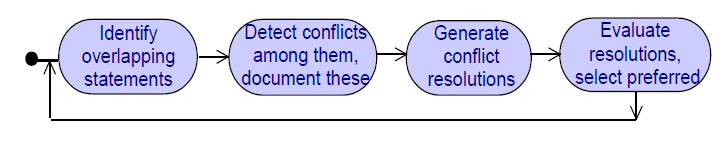
\includegraphics[width=0.5\textwidth]{img/requirements/conflicts.png}
      \caption{Managing conflicts}
      \label{fig:conflicts}
\end{figure}
Analizzando nel dettaglio la figura \ref{fig:conflicts} abbiamo:
\begin{enumerate}
      \item \textbf{identificare gli statement sovrapposti}: 
            Nella fase di sovrapposizione/overlap indichiamo il riferimento a
            termini o fenomeni comuni e sono le precondizioni del conflitto.
      \item \textbf{identificazione e documentazione dei conflitti tra gli statement}: 
            La fase di riconoscimento può essere fatta informalmente, tramite
            euristiche sulle categorie dei requisiti in conflitto, o formalmente.
            Il riconoscimento deve essere documentato per una successiva risoluzione
            e analisi dell'impatto. Si usano strumenti come l'\textbf{interaction
                  matrix} che presenta su righe e colonne gli statement e
            negli incroci indica:
            \begin{equation}
                  M[s_i,s_j] = \begin{cases}
                        1    & \text{ conflitto}                  \\
                        0    & \text{ nessun overlap}             \\
                        1000 & \text{ overlap ma senza conflitto} \\
                  \end{cases}
            \end{equation}
            Avendo, per ogni statement $S_i$, indicando con $S_i$ la riga/colonna
            corrispondente (sono uguali):
            \begin{equation}
                  conflicts(S_i) = \left(\sum_{s \ \in \ S_i} s \right) \mod 1000
            \end{equation}
            \begin{equation}
                  nonConflictingOverlaps(S_i) = \left\lfloor \sum_{s \ \in \
                        S_i} s / 1000 \right\rfloor
            \end{equation}
      \item \textbf{genera diverse risoluzioni ai conflitti}: 
            La terza fase consiste nell'esplorare tutte le soluzioni per la risoluzione
            dei conflitti, questa si effettua nel seguente modo:
            \begin{itemize}
                  \item Esplorare prima più risoluzioni, generate tramite tecniche
                        di elicitation e usando tattiche di risoluzione dei conflitti:
                        \begin{itemize}
                              \item Evitare condizioni a contorno.
                              \item Ripristinare statement in conflitto.
                              \item Indebolire gli statement in conflitto.
                              \item Non considerare statement a bassa priorità.
                              \item Approfondire source e target del conflitto.
                        \end{itemize}
                  \item Confrontare, selezionare e concordare soluzioni possibili.
            \end{itemize}
            Si trasformano quindi statement in conflitto in nuovi requisiti.
      \item \textbf{valuta le risoluzioni ai conflitti e scegli la migliore}: 
            Nella quarta fase si usano vari criteri per la scelta:
            \begin{itemize}
                  \item Contributo a requisiti non funzionali critici.
                  \item Contributo alla risoluzione di altri conflitti e rischi.
                  \item Applicazione dei principi di risk analysis.
            \end{itemize}
\end{enumerate}
La parte di \textbf{Requirements prioritization} consiste nel fornire ai vari
requisti una prioritization, per vari scopi:
\begin{itemize}
      \item Risoluzione dei conflitti.
      \item Limitazioni delle risorse.
      \item Sviluppo incrementale.
      \item Ri-pianificazione a causa di problemi imprevisti.
\end{itemize}
La priorità sui requisiti si può esprimere tramite:
\begin{enumerate}
      \item \textbf{Livelli ordinati} di uguale priorità, in un piccolo numero.
      \item \textbf{Livelli relativi} come ad esempio \textit{maggiore di}.
      \item \textbf{Requisiti comparabili}: stessa granularità, stesso livello di
            astrazione.
      \item \textbf{Requisiti non mutuamente dipendenti}.
      \item Un \textbf{accordo} con i vari partecipanti e stakeholder.
\end{enumerate}
Per i primi 3 principi si può utilizzare il metodo \textbf{Value-cost prioritization}:
\begin{itemize}
      \item Stimare il contributo relativo di ogni requisito all'interno del
            \textbf{valore} del progetto.
      \item Stimare il contributo relativo di ogni requisito all'interno del
            \textbf{costo} del progetto.
      \item Si rappresenta il diagramma valore-costo (figura \ref{fig:cost-value-diagram}).
\end{itemize}
\begin{figure}[!ht]
      \centering
      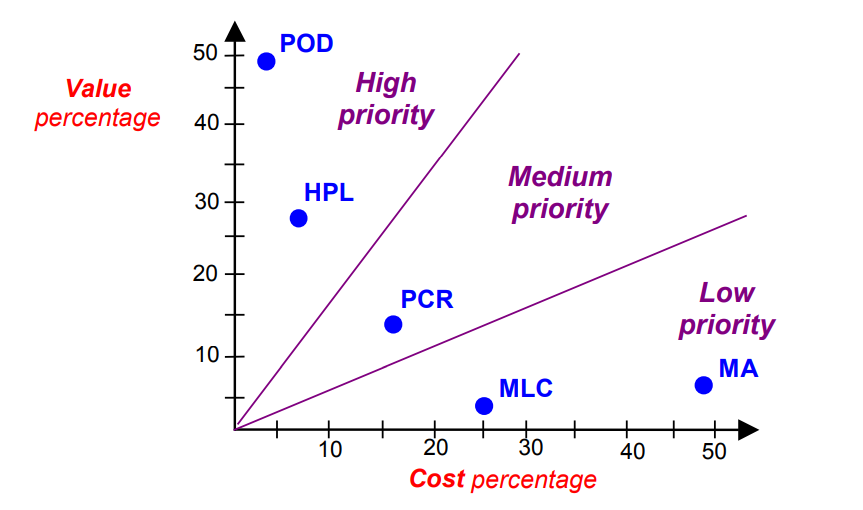
\includegraphics[width=0.5\textwidth]{img/requirements/cost-value-diagram.png}
      \caption{Diagramma Cost-value}
      \label{fig:cost-value-diagram}
\end{figure}
Si usa quindi la tecnica AHP dalla Decision Theory dove si cerca di capire in che
proporzione ogni requisito $R_i$ contribuisce al criterio $crit$, che sarà prima
il valore, $crit = value$, e poi il costo, $crit = cost$. Si hanno quindi due step:
\begin{enumerate}
      \item Si usa la comparison matrix stimando i contributi di ogni requisito sul
            criterio da studiare. Avendo $N$ requisiti:
            \begin{equation}
                  R_{i, j} = \frac{1}{R_{i, j}}, \ \text{ se} \ 1 \leq i, j \leq N
            \end{equation}
            Dalla comparison matrix si hanno dei valori, più basso è il valore
            di $R_{ij}$ allora $R_i$ contribuisce equamente insieme a $R_j$, più
            è alto il valore allora $R_i$ contribuisce molto di più rispetto a $R_j$.
      \item Si determina quanto questo si distribuisce tra tutti i requisti, tramite
            gli autovalori della matrice. Inoltre le colonne vengono normalizzate
            tramite:
            \begin{equation}
                  R_{i, j} = \frac{R_{i, j}}{\sum_i R_{i, j}}
            \end{equation}
            e aggiungendo la media sulle righe per valutare il contributo del
            requisito sul criterio.
\end{enumerate}
AHP permette di assicurare stime e rapporti consistenti.
\subsection{Specification \& documentation}
In questa fase si documentano in modo preciso i requisiti scoperti. Si descrivono
in modo preciso le feature e i concetti rilevanti per il progetto. Nel dettaglio
si definiscono in modo preciso:
\begin{itemize}
      \item Obiettivi, concetti, proprietà di dominio rilevanti, requisiti di
            sistema/software, ipotesi, responsabilità
      \item La motivazione delle opzioni scelte
      \item Un'indicazione sulle varianti e sulle evoluzioni previste
\end{itemize}
Il documento deve avere una struttura coerente. Tale documento è detto
\textbf{Requirements Document} (RD). Qualora i requisti siano stati messi online
si procede alla costruzione di un database che tiene traccia dei requisti. In
ogni caso il contenuto deve essere accessibile e comprensibile da tutte le parti
di interessate, aggiungendo spesso in allegato anche costi, workplan e piani di
delivery. Bisogna capire come effettivamente documentare i requisiti.
\subsubsection{Non-formal notation}
La prima opzione è l'utilizzo del linguaggio naturale in modo svincolato. Si ha
una forte espressività ma, in assenza di regole sulla scrittura si rischia di
produrre una sorta di romanzo, producendo qualcosa di poco gestibile. Il linguaggio
naturale inoltre può nascondere ambiguità. Usando il linguaggio naturale privo
di vincoli si hanno quindi rischi ma si può usare un linguaggio naturale strutturato,
per ottenere tale linguaggio si introducono quindi due tipi di regole:
\begin{enumerate}
      \item \textbf{Local rules}: che riguardano la scrittura del singolo requisito.
      \item \textbf{Global rules}: che riguardano le regole sulla scrittura
            dell'intero documento e sull'insieme dei requisti.
\end{enumerate}
Abbiamo però alcune regole stilistiche generali:
\begin{itemize}
      \item Scrivere pensando a chi deve leggere, che deve essere ben identificato.
      \item Spiegare cosa stiamo per scrivere prima di specificarlo nel dettaglio.
      \item Motivare le scelte.
      \item Assicurarsi che ogni concetto usato nei requisiti sia stato prima definito.
      \item Chiedersi se quanto scritto è comprensibile e rilevante.
      \item Per ogni frase/elemento del documento indicare uno e un solo requisito
            o assunzione o proprietà di dominio, evitando di mischiare troppe cose.
      \item Scrivere frasi brevi.
      \item Distinguere ciò che è obbligatorio da ciò che è desiderabile.
      \item Evitare acronimi non necessari ed evitare l'abuso del gergo informatico.
      \item Usare esempi esplicativi.
      \item Usare diagrammi o illustrazioni quando utile.
\end{itemize}
In termini di \textit{local rules} si hanno dei template per scrivere i requisiti,
usando anche un solo standard per tutti i requisti. Un esempio di template
potrebbe contenere:
\begin{itemize}
      \item Identificatore del requisito, con uno schema di naming significativo.
      \item Categoria del requisito, come ad esempio funzionale.
      \item Specifica del requisito.
      \item Criterio di fit o test di accettazione, il quale è usato quindi per
            quantità/concetti misurabili, essendo critico quindi per requisiti
            non funzionali.
      \item Fonti di elicitation.
      \item Motivazioni.
      \item Interazioni con altri requisti.
      \item Livello di priorità.
      \item Livelli di stabilità, può cambiare?.
\end{itemize}
Per le \textit{global rules} si ha una forma standard data da IEEE std-830, il
più diffuso. Si hanno varie macro-categorie a loro volta suddivise in:
\begin{enumerate}
      \item \textit{Introduzione}: si specifica anche quale parte del documento
            interessi ai vari stakeholder:
            \begin{enumerate}
                  \item Motivazioni del documento.
                  \item Scopo del prodotto.
                  \item Definizioni, acronimi, sigle e abbreviazioni.
                  \item Reference, fonti di elicitation.
                  \item Overview dell'organizzazione del documento.
            \end{enumerate}
      \item \textit{Descrizione generale}
            \begin{enumerate}
                  \item Prospettive del prodotto.
                  \item Funzionalità principali.
                  \item Caratterizzazione degli utenti.
                  \item Vincoli generali sull'ambiente (che non possono esse
                        modificati ma con i quali si deve integrare il prodotto).
                  \item Assunzioni sul prodotto e dipendenze del prodotto.
                  \item Ripartizione dei requisti.
            \end{enumerate}
      \item \textit{Requisiti specifici} usando magari il template visto prima.
            Si hanno quindi varie categorie di requisiti che articolano le varie
            sezioni del capitolo:
            \begin{enumerate}
                  \item Requisiti funzionali, che a sua volta può avere
                        un'organizzazione interna in base a vari fattori.
                  \item Requisiti per l'interfaccia esterna.
                  \item Requisiti per le prestazioni.
                  \item Vincoli di progettazione.
                  \item Attributi di qualità del software
                  \item Altri requisiti
            \end{enumerate}
      \item Appendice.
      \item Indice.
\end{enumerate}
Una variante per il template VOLERE dove si hanno sezioni esplicite per proprietà
del dominio, costi, rischi, piano di lavoro di sviluppo etc$\dots$

Il requirements document può essere dislocato in diversi posti, per esempio:
la sezione della descrizione generale può essere messa sul repository, mentre
la sezione dei requisiti specifici potrebbe essere su Trello.
\subsubsection{Semi-formal notation}
Si hanno anche opzioni aggiuntive oltre al linguaggio naturale. Una prima
alternativa sono i diagrammi, dove si ha una notazione semi-formale, in quanto
si ha una sintassi formale essendo i vari diagrammi formalmente definiti ma
l'interpretazione degli stessi può comunque essere ambigua.

Un diagramma può semplificare  quanto scritto e rappresentare il tutto in modo
compatto. L'uso di diagrammi permette di ottenere un metodo di comunicazione più
semplicemente e viene usato per aspetti specifici del sistema.

I diagrammi sono tra loro complementari ma hanno anche delle intersezioni tra di
loro e anche con il testo e tutto deve comunque restare coerente. Si rischia di
introdurre inconsistenze.

Si hanno alcune regole di consistenza per i diagrammi che vengono usate da diversi
strumenti per verificare la consistenza tra i vari diagrammi.

Uno degli standard per la modellazione di diagrammi: \textbf{Unified Modeling
      Language} (UML). Al suo interno si hanno, con regole di coerenza tra essi:
\begin{itemize}
      \item Class diagrams
      \item Use case diagrams
      \item Sequence diagrams
      \item State diagrams
\end{itemize}
In conclusione, i diagrammi hanno il vantaggio di essere in grado di dare una
buona panoramica sulla struttura/comportamento, sono facili da trasmettere e
comprendere. Sono inoltre supportati da vari tool di analisi.

Il contro è sempre la specifica ambigua semi-formale che può anche limitare
l'analisi degli stessi. Inoltre si concentrano solo su aspetti funzionali e
strutturali.

Si hanno anche gli state-chart per la descrizione di sistemi paralleli che usano
la semantica interleaving ovvero per 2 transizioni che si attivano nello stesso
stato, una viene presa dopo l'altra, in modo non deterministico.
\paragraph{Problem diagram (context diagram)}
Un primo esempio di digramma utilizzato è il \textbf{problem diagram}
\ref{fig:problemDiagram}, il quale descrive i requisiti a livello di sistema.

In questo diagramma si descrive il problema che si vuole risolvere, mostrando le
componenti del sistema e le loro interazioni. Si può specificare testualmente un
requisito e riferirlo alle componenti del sistema citate nel requisito, che è
posto in un ellisse tratteggiato. Posso avere riferimenti e vincoli sulle
componenti a partire dal requisito. Tutte le interazioni sono decorate con gli
eventi che sono rilevanti per l'interazione con il produttore dell'evento indicato
tramite le maiuscole e il nome dell'evento, a loro volta separati da “!”.

Ogni componente del sistema è indicata tramite un rettangolo in cui è presente
una doppia linea a sinistra. Il sistema comunica con diversi elementi
dell'ambiente, indicati da rettangoli.

Con questo tipo di diagramma si cattura il contesto del requisito, legando
componenti dell'ambiente e componenti del sistema, tramite specifici eventi.
Si identificano a colpo d'occhio gli elementi rilevanti per un certo requisito.

\begin{figure}[!ht]
      \centering
      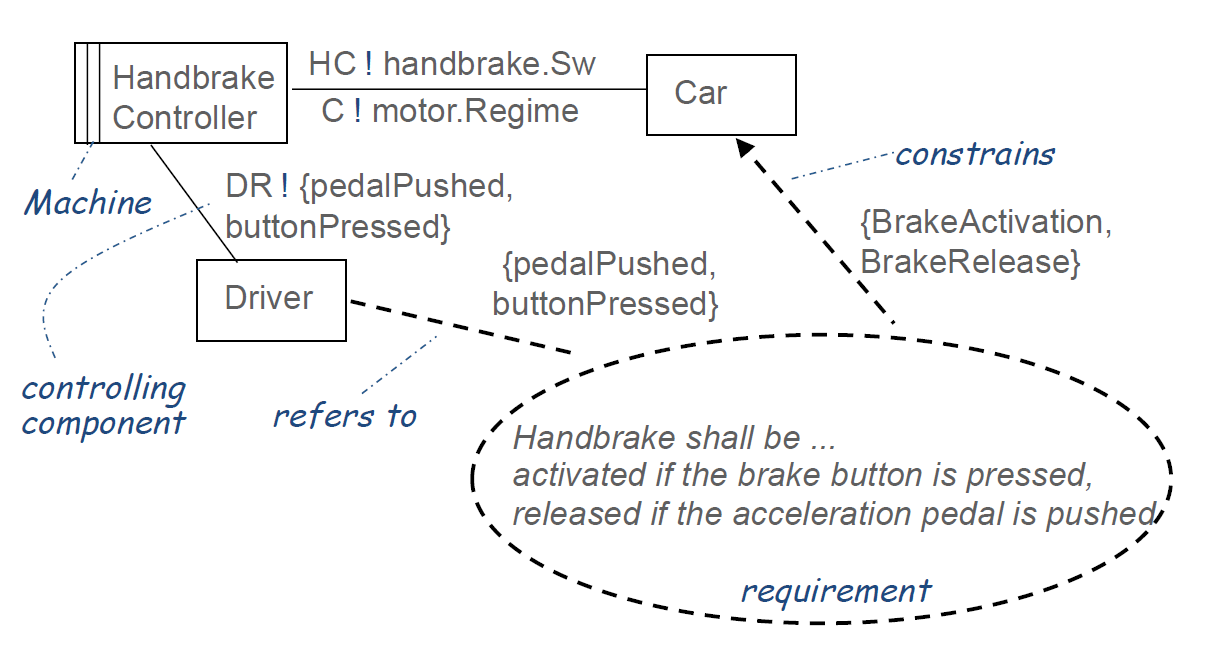
\includegraphics[width = 0.5\textwidth]{img/requirements/PD.png}
      \caption{Esempio di Problem Diagram}
      \label{fig:problemDiagram}
\end{figure}

Questa rappresentazione può prendere la forma di veri e propri pattern detti
\textbf{problem pattern} per semplificare la rappresentazione. Si ottengono i
\textbf{frame diagrams} (fig \ref{fig:frame-diagram}), che hanno la stessa
rappresentazione dei problem diagram con la differenza che si ha qualche informazione
in più, come:
\begin{itemize}
      \item \textbf{Tipo di componente}: indicato con un quadratino in basso a
            destra nel rettangolo della componente, specificato da una lettera:
            \begin{itemize}
                  \item C: causal, causa-effetto
                  \item B: biddable, non predicibile
                  \item X: lexical, lessicale, specifica artefatti
            \end{itemize}
      \item \textbf{Tipo di evento} (posto) dopo il “!” sopra descritto,
            specificato da una lettera:
            \begin{itemize}
                  \item C: causal, diretta conseguenza di altri eventi
                  \item E: event, che non sono diretta conseguenza ma che sono
                        prodotti in modo spontaneo
                  \item X: lexical, dati che vengono utilizzati per produrre
                        qualcosa
            \end{itemize}
\end{itemize}
Tali pattern vengono istanziati nei vari casi specifici.
\begin{figure}[!ht]
      \centering
      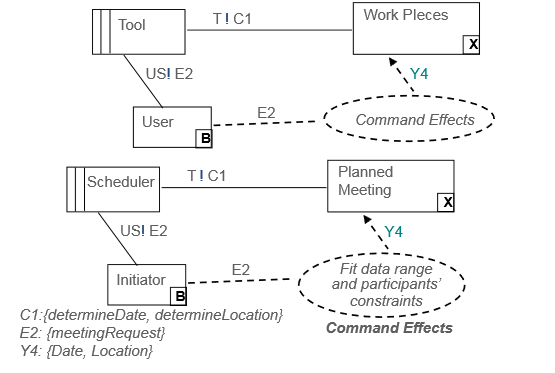
\includegraphics[width = 0.5\textwidth]{img/requirements/frame-diagram.png}
      \caption{Esempio di Frame Diagram}
      \label{fig:frame-diagram}
\end{figure}
\paragraph{Diagrammi ER}
Un altro diagramma tipico è quello ER per specificare entità che entrano in gioco
in certi aspetti dei requisiti, specificandole in modo schematico. Si usano anche
diagrammi di dominio, di classe etc$\dots$, non descrivendo più comportamenti
ma strutture, domini etc$\dots$
\paragraph{Diagrammi SADT}
I \textbf{SADT diagrams} permettono di specificare il comportamento di alcune
attività scomponendolo e aggiungendo varie informazioni. Possiamo avere due tipi
di diagrammi:
\begin{enumerate}
      \item \textbf{Actigram} \ref{fig:actigram}: sono di tipo \textit{activity-driven}
            e si concentrano sulle attività e sul mostrare le dipendenze tra le
            attività in termini di dati. Le attività sono indicate dentro
            rettangoli e si hanno una serie di frecce che a seconda della direzione
            variano il significato:
            \begin{itemize}
                  \item $\to$ (in entrata all'attività) per l'input di dati.
                  \item $\to$ (in uscita dall'attività) per l'output di dati.
                  \item $\downarrow$ per il data/event controlling, ovvero dati
                        o eventi che controllano il comportamento dell'attività,
                        sono magari aspetti di configurazione etc$\dots$ che
                        influenzano l'attività.
                  \item $\uparrow$ per l'unità che processerà l'attività, questa
                        può essere opzionale.
            \end{itemize}
            \begin{figure}[!ht]
                  \centering
                  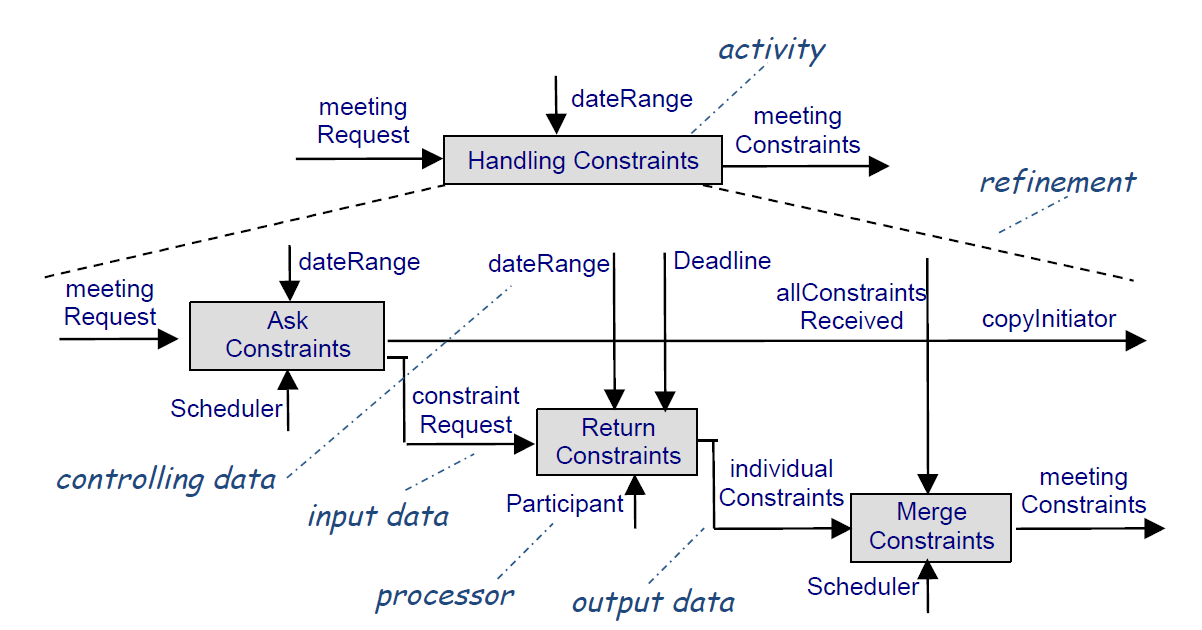
\includegraphics[width = 0.5\textwidth]{img/requirements/actigram.png}
                  \caption{Actigram}
                  \label{fig:actigram}
            \end{figure}
      \item \textbf{Datagram} \ref{fig:datagram}: sono di tipo \textit{data-driven},
            si concentrano sui dati e mostrano le dipendenze tra i dati in termini
            di attività. I dati sono indicate dentro rettangoli e si hanno una
            serie di frecce che a seconda della direzione variano il significato:
            \begin{itemize}
                  \item $\to$ (in entrata al dato) per l'input di attività che
                        producono il dato.
                  \item $\to$ (in uscita dal dato) per l'output di attività verso
                        le quali serve il dato.
                  \item $\downarrow$ per le attività di validazione del dato.
                  \item $\uparrow$ per le risorse necessarie a memorizzare e
                        gestire il dato.
            \end{itemize}
            \begin{figure}[!ht]
                  \centering
                  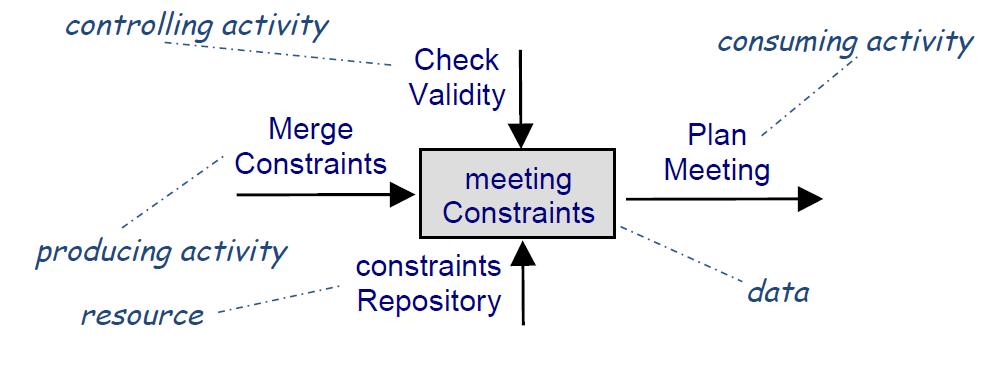
\includegraphics[width=0.5\textwidth]{img/requirements/datagram.png}
                  \caption{Datagram}
                  \label{fig:datagram}
            \end{figure}
\end{enumerate}
La coerenza tra di due diagrammi è fondamentale avendo una rapporto di dualità
tra essi quindi i dati e le attività presenti in uno devono apparire anche
nell'altro.

Questo strumento si prestano a documentare workflow molto semplici. In ogni caso:
\begin{itemize}
      \item Ogni attività deve avere un input e un output.
      \item Tutti i dati devono avere un produttore e un consumatore.
      \item I dati I/O di un'attività devono apparire come dati I/O delle
            sotto-attività.
      \item Ogni attività in un datagramm deve essere definita in un actigramma.
\end{itemize}
\paragraph{Dataflow diagram}
I \textbf{Dataflow diagram} \ref{fig:dataflow-diagram} cattura tutte le operazioni
di sistema collegate dalla dipendenza dei dati, corrisponde ad un actigram più
semplice ma meno espressivo. Si definiscono:
\begin{itemize}
      \item \textbf{Ovali}: per i componenti.
      \item \textbf{Frecce}: specificano i flussi dei dati.
\end{itemize}
\begin{figure}[!ht]
      \centering
      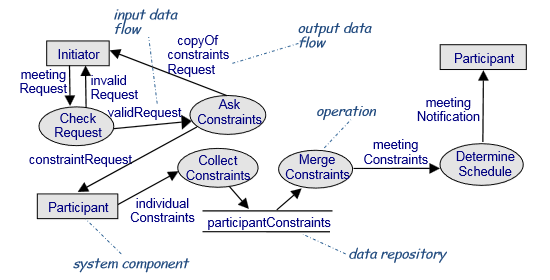
\includegraphics[width=0.5\textwidth]{img/requirements/dataflow-diagram.png}
      \caption{Dataflow diagram}
      \label{fig:dataflow-diagram}
\end{figure}
\paragraph{Use case Diagram}
Un altro diagramma classico è lo \textbf{use case diagram} per visualizzare i
requisiti identificati, che prendono forma di casi d'uso con gli attori che
partecipano allo svolgimento dei requisiti.
\paragraph{Event trace diagrams}
Un altro strumento utile nella definizione di workflow è l'\textbf{event trace
      diagrams} \ref{fig:etd}, ovvero i diagrammi di sequenza. Se ne hanno vari
tipi con sintassi più o meno ricche ma in generale si hanno $N$ elementi che
partecipano all'esecuzione che viene mostrata visualmente tramite richieste e
risposte, sincrone o meno, che vengono indicate cronologicamente dall'alto al basso.
\begin{figure}[!ht]
      \centering
      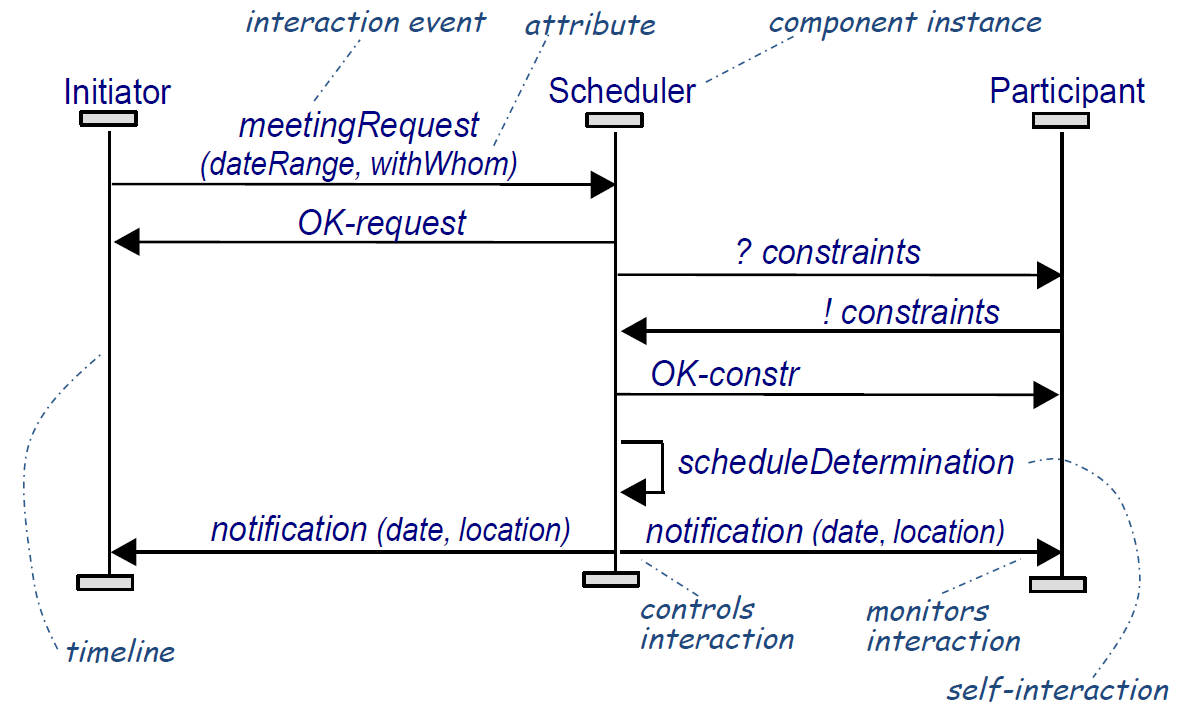
\includegraphics[width=0.5\textwidth]{img/requirements/etd.png}
      \caption{Event trace diagrams}
      \label{fig:etd}
\end{figure}
Questa visualizzazione compatta aiuta nel momento in cui il linguaggio naturale
diventa troppo complesso e verboso per spiegare una certa sequenza di azioni.
\paragraph{State machine diagram}
Un altro diagramma usato è lo \textbf{state machine diagram} \ref{fig:smd} per
mostrare in quali stati un particolare elemento si trova e quali transizioni/eventi
modificano i suoi stati. Questi diagrammi sono utili in quanto in modo compatto
rappresentano il ciclo di vita di una certa componente, facilitando la creazione
del sistema.
\begin{figure}[!ht]
      \centering
      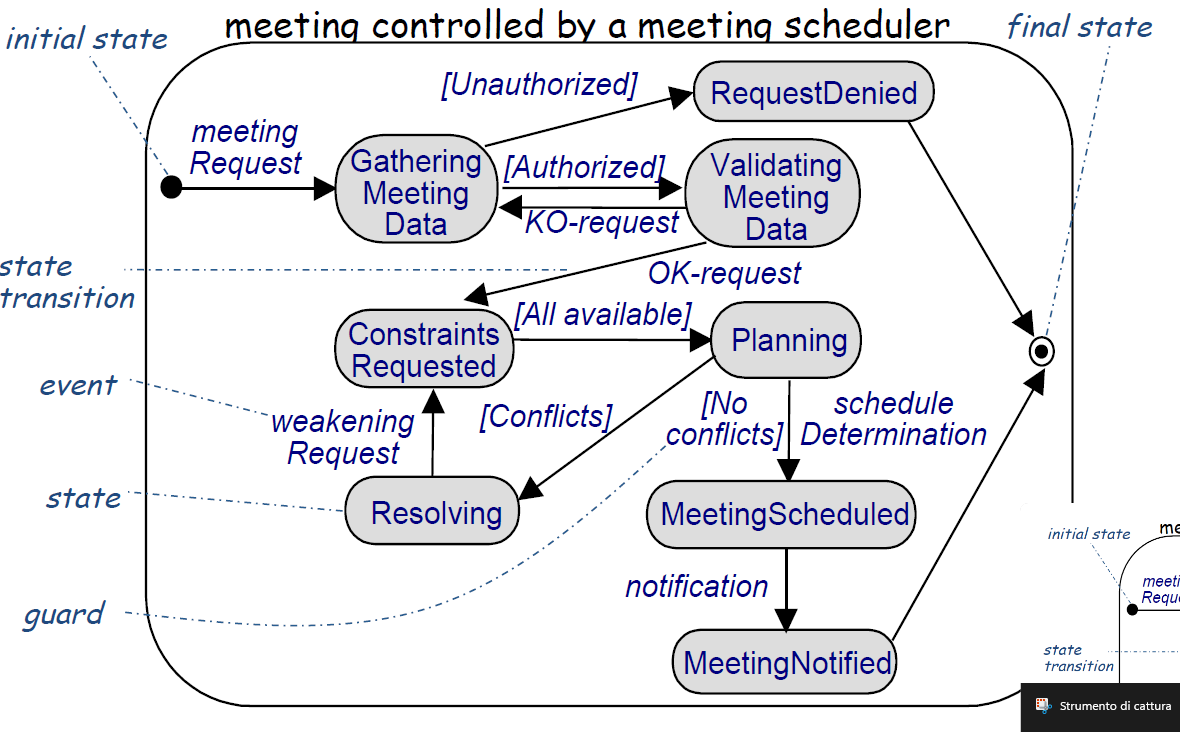
\includegraphics[width=0.5\textwidth]{img/requirements/smd.png}
      \caption{State machine diagram}
      \label{fig:smd}
\end{figure}
\paragraph{R-net diagram}
Come altro diagramma abbiamo il \textbf{R-net diagram} \ref{fig:r-net-diagram}
che permette di mostrare come reagisce un sistema in base ad un certo stimolo.
È quindi un albero che parte con uno stimolo, dopo il begin, posto in un esagono
e si sviluppa in base alle varie alternative in corrispondenza di punti di
decisione (indicati come pallini). Nei rettangoli si hanno le azioni che sono
svolte in conseguenza allo stimolo.
\begin{figure}[!ht]
      \centering
      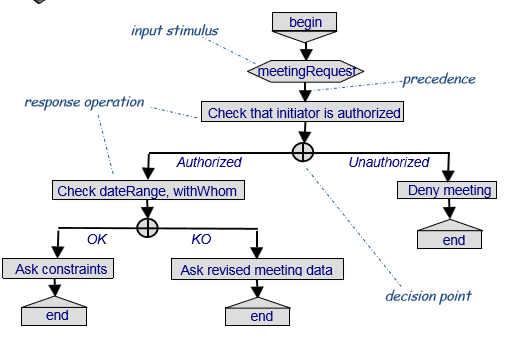
\includegraphics[width=0.5\textwidth]{img/requirements/r-net-diagram.png}
      \caption{R-net diagram}
      \label{fig:r-net-diagram}
\end{figure}
\subsubsection{Formal notation}
Si ha quindi la necessità di una semantica formale per rappresentare aspetti
mission - critical. Questo non viene garantito dai diagrammi, ma si hanno
linguaggi appositi la cui creazione/gestione/documentazione è assai costosa per
cui vengono usati solo in casi estremamente specifici.

Si parla sia di sintassi che di semantica. Tali definizioni formali permettono
di avere un compilatore  che sia in grado di processare tali specifiche. Si ha
quindi un livello di precisione alto e non si ha ambiguità, permettendo analisi
di consistenza e coerenza delle specifiche.

Una sintassi/semantica formale è quella data dalla logica proposizionale e dalle
formule ben formate. Si ha quindi un linguaggio basato sui connettori logici e
sulle regole per avere formule ben formate.

Ogni statement può quindi essere interpretato con il valore di verità con le
regole definite dalla logica e dalle tabelle di verità. Si vede quanto produrre
tutto questo per un progetto enorme risulti costoso. Vengono quindi usate le
classiche regole di inferenza. Si usa anche la logica predicativa del primo ordine.

Un altro strumento usato è la logica temporale con l'aggiunta dei connettivi
temporali.

Si ha un approccio formale anche su specifiche state-based dove si specifica in
modo formale cosa sia l'insieme degli stati che il sistema può attraversare e
come delle operazioni modificano lo stato.

Si usano linguaggi come $Z$ basati sulla teoria degli insiemi. Ogni stato è
caratterizzato da pre e post condizioni e si studiano le regole in termini di
invarianti che lo stato deve soddisfare.

Con $Z$ si producono schemi dove si specifica un certo elemento, gli attributi di
stato con $P$ che indica l'insieme delle parti che precede il tipo. Si ha poi un
invariante per gli attributi che definisce l'elemento. Si ha quindi una
caratterizzazione basata sulla teoria degli insiemi. Si hanno sia tipi primitivi
che strutturati. Per definire invece le modifiche che portano a nuovi stati.

Sopra si hanno tutti gli elementi coinvolti nell'operazione. La prima linea della
parte sotto è per le precondizioni, quella sotto per le post-condizioni, entrambe
con la notazione insiemistica. Gli elementi sono inoltre così decorati:
\begin{itemize}
      \item stateVar?:Type indica una variabile di input.
      \item stateVar':Type indica una variabile di output mutevoli.
      \item stateVar!:Type indica una variabile di output esterne e non mutevoli
      \item $\Delta$ schema indica che si ha una modifica delle variabili importate
            dallo schema.
      \item $\Xi$ schema indica che non si ha una modifica delle variabili importate
            dallo schema.
\end{itemize}
Il cambiamento di stati ben definito diventa studiabile e simulabile, studiando
lo spazio di comportamenti del sistema a questo livello di astrazione,
individuando problemi che porterebbero alla correzione di requisiti. Si può avere
anche l'inclusione di più schemi. Con questa specifica state-based si hanno vari
vantaggi:
\begin{itemize}
      \item Automazione semplice grazie a logica, matematica discreta, studio
            degli invarianti etc$\dots$
      \item Ottimi meccanismi di strutturazione per comporre unità e strutture
            stati complessi.
      \item Permette l'analisi automatica: type checking, consistency checking,
            etc$\dots$
\end{itemize}
Di contro non permette di studiare altro se non aspetti funzionali e non ha
un'historical referencing.

Si ha anche una specifica algebrica per formalizzare le leggi che compongono le
operazioni, viste come funzioni matematiche senza esplicita nozione di stato.
Si ha invece un system history avendo una “traccia” delle operazioni.

Si hanno tipi di dato astratti, parametrizzazione, equazioni condizionali e funzioni
parziali. Si hanno tre tipi di operazione:
\begin{enumerate}
      \item Modifiers, per produrre qualsiasi istanza di concetto mediante
            composizione con altri modifier.
      \item Generators, ovvero un sottoinsieme minimo di modifiers per generare
            qualsiasi istanza di concetto con un numero minimo di composizioni.
      \item Obsevers, per ottenere informazioni pertinenti su qualsiasi istanza
            di concetto.
\end{enumerate}
Spesso si hanno funzioni ricorsive.

Come vantaggi si hanno:
\begin{itemize}
      \item Analisi automatica efficiente.
      \item Specifiche eseguibili.
      \item Ricchi meccanismi di strutturazione (import, ereditarietà $\dots$).
\end{itemize}
Di contro si ha una limitata potenza espressiva (solo equazioni senza historical
referencing) e una forte vicinanza alla programmazione (comportando difficoltà
di validazione in caso, ad esempio, di ricorsioni).

Tendenzialmente i limiti della notazione formale sono sempre questi (oltre alla
difficoltà di lettura/scrittura), anche se permette alta precisione, pochi difetti
di specifica, analisi sofisticata (anche automatica), generazione di artefatti
come test cases, codice etc$\dots$.

Ricapitolando:
\begin{itemize}
      \item Il linguaggio naturale “puro” non è un'opzione.
      \item Il linguaggio naturale strutturato è quello più usato.
      \item I diagrammi sono un'ottima aggiunta al linguaggio naturale.
      \item La notazione formale è usata in rare circostanze.
\end{itemize}
\subsection{Validation \& verification}
Siamo quindi all'ultima delle quattro fasi, dove bisogna validare i requisiti.
Si hanno vari approcci per validare la qualità dei requisiti:
\begin{itemize}
      \item \textbf{Analisi e revisione dei singoli requisiti}: è manuale e
            costoso in termini di tempo ma si può sempre fare.
      \item \textbf{Interrogare il database delle specifiche}: è automatico ma
            non controlla la qualità di tutti.
      \item \textbf{Usare le specification animation}: servono dei requisiti
            eseguibili, buono per trovare dei bug.
      \item \textbf{Check formale}: richiede requisiti specificati in modo
            formale e può rivelare tutti i bug.
\end{itemize}
\subsubsection{Analisi e revisione dei singoli requisiti}
Questo è sempre applicabile ma va fatto manualmente impiegando molto tempo. La
prima operazione consiste nel ricercare errori nel Requirements Document. Spesso
questi sono gli errori più numerosi e pericolosi e possono avere varia natura:
\begin{itemize}
      \item Omissione
      \item Contraddizione
      \item Inadeguatezza
      \item Ambiguità
      \item Incommensurabilità
      \item Rumore
      \item Eccesso di specificità
      \item Scarsa struttura
      \item Opacità
\end{itemize}
Bisogna quindi individuare quanti più problemi possibili nel Requirements Document,
validarli (vedendo se le informazioni utili sono necessarie), verificarli (vedendo
se sono completi e consistenti) e confermare non ambiguità, misurabilità,
fattibilità, buona struttura, etc$\dots$

Bisogna quindi fare il report dei problemi, analizzarne la causa e correggerli.
Questa operazione viene fatta selezionando personale che ispeziona il Requirements
Document individualmente per poi confrontare le opinioni. Tali persone possono
essere interne ai project members o recensori esterni. Questo viene spesso fatto
anche per il codice sorgente e quindi si è mostrato che è empiricamente utile
anche per le revisioni del Requirements Document.

La revisione può essere effettuata in vari modi:
\begin{itemize}
      \item \textbf{Free mode}: senza direttiva su cosa cercare e dove.
      \item \textbf{Checklist-based}: indicando una lista di cose da controllare.
      \item \textbf{Process-based}: dove si hanno ruoli specifici, procedure
            dettagliate, tecniche di analisi etc$\dots$, rendendo questa la
            modalità più efficace.
\end{itemize}
Il report deve essere fatto in modo informativo e accurato, senza opinioni o
commenti offensivi. Ovviamente le revisione deve essere fatta possibilmente da
personale diverso da quello che scrive il Requirements Document e tale personale
deve rappresentare tutti gli stakeholder con le varie conoscenze pregresse.

A livelli di tempo il controllo deve essere effettuato ne troppo presto ne troppo
tardi ma con incontri ripetuti per ottenere la massima efficacia.

Ci si deve inoltre concentrare sulle parti più critiche, che devono essere meglio
analizzate. Dal punto di vista delle checklist se ne hanno diverse:
\begin{itemize}
      \item \textbf{Defect-driven}: lista dei difetti tipici, strutturate tramite
            un elenco di domande generiche.
      \item \textbf{Quality-specific}: lista più specializzata di quella
            defect-driven, specializzandosi su requisiti non funzionali.
      \item \textbf{Domain-specific}: lista specializzata nei concetti e nelle
            operazioni di dominio per aiutare nella ricerca dei difetti.
      \item \textbf{language-based}: lista specializzata nei costrutti legati ai
            linguaggi. In questa parte si analizzano anche i diagrammi, si
            analizzano anche linguaggi di specifica come $Z$.
\end{itemize}
Si usano anche delle \textbf{checking decision tables} che hanno in input $N$
condizioni booleane ($\{T, F\}$) e una serie di eventi che si hanno in conseguenza
allo stato delle condizioni, specificando se accadono o meno. Si ha che se il
numero di combinazione dei vari casi specificati dalle condizioni in input è minore
$2^N$ (se ho meno colonne del dovuto nella tabella di verità) allora mancano dei
casi da analizzare mentre se è maggiore si hanno dei casi ridondanti.

Questo tipo di analisi è quindi applicabile potenzialmente alla ricerca di ogni
difetto (anche se non si ha garanzia di riconoscerli tutti, per quanto critici,
anche se con un mix delle tecniche spiegate si raggiungono ottimi risultati).
I costi restano elevati sia in termini monetari che di tempo.
\subsubsection{Interrogare il database delle specifiche}
Questo, a livello superficiale, può essere fatto in modo automatico ma è appunto
un check parziale. Questa tecnica è specifica per casi particolari, dove le
specifiche sono memorizzate in un database. Le query acquisiscono controlli per
la coerenza strutturale intra o inter-diagrammi e tali query possono essere
generate a partire dal diagramma ER. Si parla anche di press-button mode quando
si ha una lista di query prescritte per la violazione delle regole di coerenza
standard.
\subsubsection{Usare le specification animation}
Sono ottime per i non esperti per identificare i problemi ma sono limitate alle
specifiche “eseguibili”, consentendo quindi solo un check parziale. Si vuole
verificare l'adeguatezza dei requisiti rispetto alle effettive necessità. Si
hanno due approcci tipici:
\begin{enumerate}
      \item Mostrare una vera interazione con lo scenario. In questo caso gli
            strumenti di “promulgazione” possono essere utilizzati sul diagramma
            NET ma ovviamente si ha il problema del range di copertura dei
            problemi dato dallo scenario.
      \item Usare tool per l'animazione delle specifiche. Si procedere generando
            un modello eseguibile e si procede alla simulazione (provvedendo a
            stimoli e vedendo il risultato) per poi raccogliere il feedback
            dell'utente. Si può avere:
            \begin{itemize}
                  \item Formato testuale, con comandi di input e poi esecuzione.
                  \item Formato a diagrammi, con un input che comporta l'evoluzione
                        di parti del diagramma.
                  \item Scena vera e propria con pannelli per l'input e scene animate
                        nell'ambiente scelto.
            \end{itemize}
\end{enumerate}
In ogni caso si ha un approccio model-based, si parla infatti di model-driven
development (sviluppando fin dall'inizio modellando il comportamento del software),
e si hanno vari tool per i vari linguaggi di specifica (SCR, LTSA etc$\dots$).

Tra i vantaggi si hanno:
\begin{itemize}
      \item È modo migliore per verificare l'adeguatezza rispetto ai bisogni reali,
            all'ambiente reale.
      \item Permette la facile interazione con gli stakeholder secondo la filosofia
            WYSIWYC (What You See Is What You Check)
      \item Estendibile per animare controesempi generati da altri strumenti.
      \item Le animazioni possono essere riusate per altri scenari.
\end{itemize}
Si hanno anche contro:
\begin{itemize}
      \item Si richiede un'attenta progettazione degli scenari che possono presentare
            problemi e non si ha garanzia di non trascurare problemi critici.
      \item Necessita specifiche formali.
\end{itemize}
\subsubsection{Check formale}
Questo permette di individuare un ottimo range di problemi ma richiede la notazione
formale, costosa, ed esperti. Si possono avere check sintattici per il linguaggio
(di specifica come $Z$) usato. Si può avere anche un check di completezza e
consistenza grazie al linguaggio e la verifica di proprietà:
\begin{itemize}
      \item \textbf{Algoritmiche}: tramite model checking, per controllare se un modello di
            comportamento soddisfa un requisito, una proprietà di dominio o un
            presupposto, cercando violazione delle varie proprietà e generando
            eventuali controesempi o comunque specifiche della violazione
            (fattori utili nel debugging). Si possono controllare:
            \begin{itemize}
                  \item Raggiungibilità, tramite un grafo di raggiungibilità.
                  \item Proprietà di safety, producendo controesempi.
                  \item Proprietà di liveness, che comporta che una condizione
                        potrebbe non essere mai raggiunta in caso di risposta
                        negativa del check.
            \end{itemize}
            I \textbf{vantaggi} del model checking sono:
            \begin{itemize}
                  \item Check completamente automatici.
                  \item Ricerca esaustiva che porta a non tralasciare alcun
                        difetto.
                  \item L'uso di controesempi può rivelare errori sottili,
                        difficili da individuare altrimenti.
                  \item È facile da abbinare agli animators per visualizzare le
                        tracce.
                  \item È sempre più usato per progetti mission critical.
            \end{itemize}
            Ma si hanno anche dei \textbf{contro}:
            \begin{itemize}
                  \item Si rischia di avere un'esplosione combinatoria degli
                        stati da analizzare comportando l'impossibilità di essere
                        eseguito per sistemi molto grossi.
                  \item I controesempi possono essere complessi da capire e
                        mostrano solo i sintomi dei problemi, non le cause.
            \end{itemize}
      \item \textbf{Deduttive tramite theorem proving}. Il theorem proving viene
            usato per generare nuove specifiche tramite le regole di inferenza
            della logica. Si studiano le conseguenze logiche delle specifiche
            evidenziando eventuali inconsistenze in un processo generalmente
            iterativo per:
            \begin{itemize}
                  \item Fornire, accettare o rifiutare i lemmi.
                  \item Suggerire strategie di prova.
            \end{itemize}
            Si hanno diversi \textbf{pro}:
            \begin{itemize}
                  \item Solidità e completezza del sistema formale utilizzato
                        avendo che ogni conclusione è corretta e che ogni
                        conclusione corretta è derivabile.
                  \item Mostra specifiche incoerenti, conseguenze inadeguate.
                  \item Può essere usato per sistemi molto grandi, gestendo una
                        gran mole di dati tramite l'induzione.
            \end{itemize}
            ma si hanno ovviamente dei \textbf{contro}:
            \begin{itemize}
                  \item È di uso difficile e richiede personale esperto.
                  \item Non produce controesempi.
            \end{itemize}
\end{itemize}
Si hanno, per i check di consistenza quando servizi o comportamenti sono
specificati come relazioni I/O capendo:
\begin{itemize}
      \item Se la relazione è una funzione (per isolare eventuali non determinismi)
      \item Se la funzione è totale e quindi in grado di specificare ogni input
\end{itemize}
\subsection{Requirements changes}
I cambiamenti dei requisiti sono assai frequenti e quindi vanno gestiti. Si hanno
infatti varie iterazioni delle 4 fasi sopra descritte, formando la spirale.

Si hanno cambiamenti organizzativi, nuove normative, nuove opportunità,
tecnologie alternative, priorità e vincoli in evoluzione oltre ad una migliore
comprensione delle caratteristiche, dei punti di forza, dei limiti e dei difetti
del sistema. Un altro aspetto riguarda il problema di gestione delle informazioni,
in merito al mantenimento della coerenza, propagazione delle modifiche, controllo
delle versioni etc$\dots$

La gestione dei cambiamenti di requisito consiste quindi nel processo di
anticipazione, valutazione, accordo e propagazione dei cambiamenti nelle varie
parti del Requirements Document.

Innanzitutto bisogna identificare i cambiamenti probabili, valutare la probabilità
e documentarli al fine di:
\begin{itemize}
      \item Anticipare una risposta adeguata quando si verificherà il cambiamento,
            studiando eventuali dipendenze tra i requisiti.
      \item Progettare l'architettura che rimanga stabile nonostante i cambiamenti.
\end{itemize}
Inoltre, associando livelli di stabilità a gruppi di statement che definiscono le
varie feature. Si punta ad avere un numero di livelli comunque ridotto e di
cercare di permettere la comparabilità, che sia qualitativa e relativa.

Si usano regole euristiche per studiare i probabili cambiamenti, concentrandosi
sui requisiti che è più facile cambino, limitando così i costi. Il livello più
alto di stabilità viene definito per quelle feature presenti in ogni estensione/
variante del sistema. Si ha che aspetti intenzionali e concettuali, così come
aspetti funzionali e obiettivi chiave, sono più stabili di aspetti operazionali
e non funzionali.

La scelta tra varie alternative rende l'oggetto della scelta poco stabile anche
perché tale scelta può essere basata su una conoscenza incompleta, presupposti
volatili o generata da risoluzione di conflitti o contromisure a vari rischi.

Quindi tali requisiti sono poco stabili.

Un altro aspetto essenziale nello studio dell'evoluzione del progetto è legato
alla gestione della \textbf{tracciabilità} (\textbf{Traceability Management}
(TM)), che non è uno studio semplice nel caso dei requisiti ma torna comodo nel
momento dei loro cambiamenti per gestire il cambiamento dell'intero progetto. Si
ha che un certo aspetto è tracciabile se e solo se si sa perfettamente:
\begin{itemize}
      \item Da dove viene
      \item Perché esiste
      \item Per cosa sarà usato
      \item Come sarà usato
\end{itemize}
Possiamo quindi dire che il Traceability Management si occupa di identificare,
documentare, recuperare la logica e l'impatto degli elementi contenuti nel
Requirements Document.

Si possono avere anche tracciamenti in merito o obiettivi specifici per determinati
requisiti, valutando l'impatto di eventuali modifiche e studiando come propagare
facilmente i cambiamenti per mantenere la coerenza ad altri elementi
dell'Requirements Document o, “scendendo di livello”, ad oggetti software.

Un aspetto centrale nel Traceability Management è rappresentato dai collegamenti
di tracciabilità tra gli elementi del Requirements Document. Tali collegamenti
vanno scoperti, memorizzati ed eventualmente recuperati. Sono bidirezionali e,
ipotizzando uno schema verticale tra le varie fasi, si hanno:
\begin{itemize}
      \item \textbf{Forward traceability}: Accessibilità dal source al target
            (che nello schema verticale sono le frecce verso il basso
            \ref{fig:traceability-diagram}). Il source motiva l'esistenza del
            target.
      \item \textbf{backward traceability}: Accessibilità dal target al source
            (che nello schema verticale sono le frecce verso l'alto
            \ref{fig:traceability-diagram})
\end{itemize}
All'interno di una stessa fase posso avere anche collegamenti (che in questo caso
non vengono direzionati a differenza dei due appena espressi e sono orizzontali).
Dipendenze tra cambiamenti di fase sono sempre rappresentatati da una linea verticale.
\begin{figure}[!ht]
      \centering
      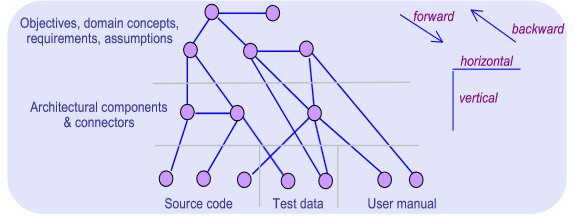
\includegraphics[width=0.5\textwidth]{img/requirements/traceability-diagram.png}
      \caption{Traceability diagram}
      \label{fig:traceability-diagram}
\end{figure}
La \textit{backward traceability} viene usata per stabilire perché un certo
elemento sia lì e da dove viene (anche ricorsivamente) mentre la \textit{forward}
per stabilire dove un elemento verrà considerato e con quali implicazioni
(anche ricorsivamente). Ricorsivamente perché posso andare indietro/avanti di
più step. Bisogna localizzare e valutare l'impatto dei cambiamenti lungo i
collegamenti orizzontali/verticali.

Elencando le varie tecniche Traceability Management, per tracciare i vari
collegamenti, si hanno:
\begin{itemize}
      \item Cross referencing
      \item Matrici di tracciabilità
      \item Feature diagrams (nel dettaglio quelli con supporto a più variant link
            type)
      \item Database di tracciabilità
      \item Database di modelli di tracciabilità
      \item Tracciabilità Specification-based
\end{itemize}
È comunque un discorso molto complesso, costoso e studiato.

Con la \textbf{tecnica di cross referencing} si seleziona ogni elemento da tracciare e
gli si assegna un nome unico. Si definisce poi lo schema di indice/tag per
collegarli lessicalmente e si configura un motore di ricerca su tale schema.
Si recuperano quindi gli elementi seguendo le catene di riferimenti incrociati,
le cross-reference chains. Un esempio banale in un documento potrebbe essere
specificare che sezione dello stesso documento andare a guardare per chiarire un
certo concetto.

Come \textbf{pro} si hanno:
\begin{itemize}
      \item La leggerezza e la disponibilità.
      \item Il supporto di ogni livello di granularità (assegnando identificatori
            a ciò che vogliamo)
\end{itemize}
Come \textbf{contro}:
\begin{itemize}
      \item Un solo tipo di collegamento, quello lessicale, privo di semantica
      \item Informazioni di tracciabilità nascoste
      \item Il costo del mantenimento dello schema di indicizzazione (anche se si ha
            un basso costo iniziale)
      \item Controllo e analisi limitate
\end{itemize}
In merito alla \textbf{matrice di tracciabilità} \ref{fig:dependency-matrix}
abbiamo che essa è la matrice di adiacenza di un grafo a singola relazione di
tracciabilità, detto \textbf{dependency graph}. In posizione ($i,j$) troviamo 1
se si ha un arco orientato tra l'item $T_i$ e l'item $T_j$ , 0 altrimenti.
Possiamo quindi dire che sulla riga i-sima troviamo gli elementi che dipendono
da $T_i$ e sulla colonna i-sima gli elementi che sono dipendenza di $T_i$.

Come \textbf{pro} si hanno:
\begin{itemize}
      \item Navigazione backward e forward.
      \item Semplice analisi dello schema (ad esempio è semplice identificare un
            ciclo di dipendenza, avendo un ciclo nel grafo).
\end{itemize}

Come \textbf{contro}:
\begin{itemize}
      \item Grafi di grandi dimensioni sono soggetti ad errori oltre ad essere
            difficilmente gestibili.
      \item Supportano un solo tipo di relazione.
      \item Dovrei creare più matrici per collegamenti tra oggetti con semantiche
            diverse.
\end{itemize}
\begin{figure}[!ht]
      \centering
      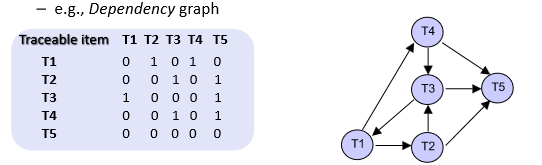
\includegraphics[width=0.5\textwidth]{img/requirements/dependency-matrix.png}
      \caption{Dependency matrix}
      \label{fig:dependency-matrix}
\end{figure}
Quest'ultimo contro può essere risolto coi \textbf{feature diagrams}
\ref{fig:feature-diagram} che sono rappresentazione grafica dei punti in comune
e delle varianti del sistema, permettendo la rappresentazione compatta di un
gran numero di varianti. Avere più varianti permette di distribuire il sistema
con un ampio numero di feature.

Nel diagramma le feature sono rettangoli e possono essere obbligatorie (con un
pallino nero) o opzionali (con un pallino bianco). Si hanno anche potenziali or
esclusivi, or non-esclusivi e and per separare in diversi modi feature in
sotto-feature. Le varie combinazioni espresse dalle feature del digramma, seguendo
la logica di opzionali o meno e delle varie suddivisioni esprimono le varianti
del progetto.
\begin{figure}[!ht]
      \centering
      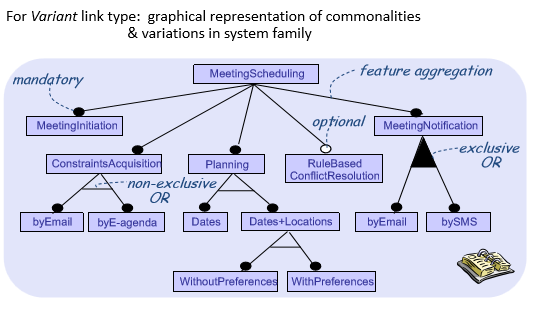
\includegraphics[width=0.5\textwidth]{img/requirements/feature-diagrams.png}
      \caption{Feature diagram}
      \label{fig:feature-diagram}
\end{figure}